\part{Celestial $\mathcal{A}$mplitudes \& CCFT}\label{part8}
% 计数器清零,每个part都要引用,除了part1
\setcounter{theorem}{0}
\setcounter{definition}{0}
\setcounter{lemma}{0}
\setcounter{sidenote}{1}
\section{Conformal basis}
QFT中利用费曼图计算散射振幅都是在动量空间下进行的,也就是选取在平面波为基底,这样做最大的好处是可以显现出平移对称性。但是在考虑天球上的散射问题时,很显然我们应当最大化利用共性对称性,所以基底应该选取为类似CFT中初级场的形式,称之为“Conformal Primary Wave Function”,这样$\mathbb{R}^{d+1,1}$上的散射振幅就有希望在这个基底下类似于CFT$_{d}$中的n点关联函数,Clifford Cheung很早就利用这个基底对一些特殊情形进行了研究\cite{Cheung:2016iub}\sn{历史上最早可以追溯到Dirac\cite{436861d5-35f6-36cf-9470-cb587eced490}}。现在顺着文献\cite{Pasterski:2017kqt}的思路来介绍这一组基底。
\subsection{Massive Scalar}
\begin{definition}[Massive Scalar Conformal Primary Wave Function]
自旋为$0$的标量场既没有$\mathbb{R}^{d+1,1}$上的$SO^\uparrow(d+1,1)$指标,也没有spinning CFT特有的张量指标,或者说处于$SO(d)$的标量表示。对于平面波,我们使用在壳动量来标记基底,现在我们使用$\Delta\in\mathbb{C},\vec{w}$来标记基底。
\begin{itemize}
	\item 在壳:
	\begin{equation}
		\left(\frac{\partial}{\partial X^{\nu}} \frac{\partial}{\partial X_{\nu}}-m^{2}\right) \phi_{\Delta}\left(X^{\mu} ; \vec{w}\right)=0
	\end{equation}
	\item 在共形变换和$SO(d+1,1)$下协变:
	\begin{equation}
		\phi_{\Delta}\left({\Lambda^{\mu}}_{\nu} X^{\nu} ; \vec{w}^{\prime}(\vec{w})\right)=\left|\frac{\partial \vec{w}^{\prime}}{\partial \vec{w}}\right|^{-\Delta / d} \phi_{\Delta}\left(X^{\mu} ; \vec{w}\right)
	\end{equation}
	这里$\vec{w}\to\vec{w}^\prime$是共形变换\footnote{注意,对于$d=2$的情形,对应的是全局共形变换,更类似于准初级场。},${\Lambda^\mu}_\nu$是诱导的Lorentz变换。
\end{itemize}
\end{definition}
后面的讨论使用Embedding形式将$\mathbb{R}^{d}$嵌入到$\mathbb{R}^{d+1,1}$的光锥,再次写下这个嵌入:
\begin{equation}
	q^\mu(\vec{w})=\left(1+|\vec{w}|^2,2\vec{w},1-|\vec{w}|^2\right),\quad q^\mu(\vec{w}^\prime)=\left|\frac{\partial \vec{w}^\prime}{\partial\vec{w}}\right|^{\frac{1}{d}}{\Lambda^\mu}_\nu q^\nu(\vec{w})
\end{equation}
粒子在壳动量$p^2=-m^2$,由于质量是固定的,抽出动量方向得到$\hat p^2=-1$,而这其实就说明$\hat p$位于unit hyperboloid space $\mathbb{H}_{d+1}$上\sn{$\mathbb{H}_{d+1}$表示$d+1$维截面曲率恒为$-1$的超曲面,Killing-Hopf定理保证这样的曲面只有这一种}。可以利用Poincar\'e half-plane对$\mathbb{H}_{d+1}$进行参数化:
\begin{equation}
	ds^2_{\mathbb{H}_{d+1}}=\frac{dy^2+d\vec{z}\cdot d\vec{z}}{y^2},\quad y>0,\vec{z}\in\mathbb{R}^d
\end{equation}
$y=0$对应$\partial\mathbb{H}_{d+1}$。$ds^2_{\mathbb{H}_{d+1}}$天然是$SO(d+1,1)$不变的,也就是在下面的变换下不变:
\begin{itemize}
	\item $\mathbb{R}^d$ translation : $\quad y^{\prime}=y, \quad \vec{z}^{\prime}=\vec{z}+\vec{a}$,\\
	\item $S O(d)$ rotation : $y^{\prime}=y, \quad \vec{z}^{\prime}=M \cdot \vec{z}$,\\
	\item dilation : $\quad y^{\prime}=\lambda y, \quad \vec{z}^{\prime}=\lambda \vec{z}$\\
	\item special conformal transformation : $y^{\prime}=\frac{y}{1+2 \vec{b} \cdot \vec{z}+|\vec{b}|^2\left(y^2+|\vec{z}|^2\right)}, \quad \vec{z}^{\prime}=\frac{\vec{z}+\left(y^2+|\vec{z}|^2\right) \vec{b}}{1+2 \vec{b} \cdot \vec{z}+|\vec{b}|^2\left(y^2+|\vec{z}|^2\right)}$
\end{itemize}
任意在在壳动量$m\hat p$可以参数化为:
\begin{equation}
	\hat{p}(y,\vec{z})=\left(\frac{1+y^2+|\vec{z}|^2}{2y},\frac{\vec{z}}{y},\frac{1-y^2-|\vec{z}|^2}{2y}\right)
\end{equation}
这其实就是在将$\mathbb{H}_{d+1}$嵌入到$\mathbb{R}^{d+1,1}$的未来光锥部分\sn{因为$\hat p^0>0$},比如$\mathbb{R}^{3,1}$的时空图就可以分层为:
\begin{figure}[H]
	\centering 
	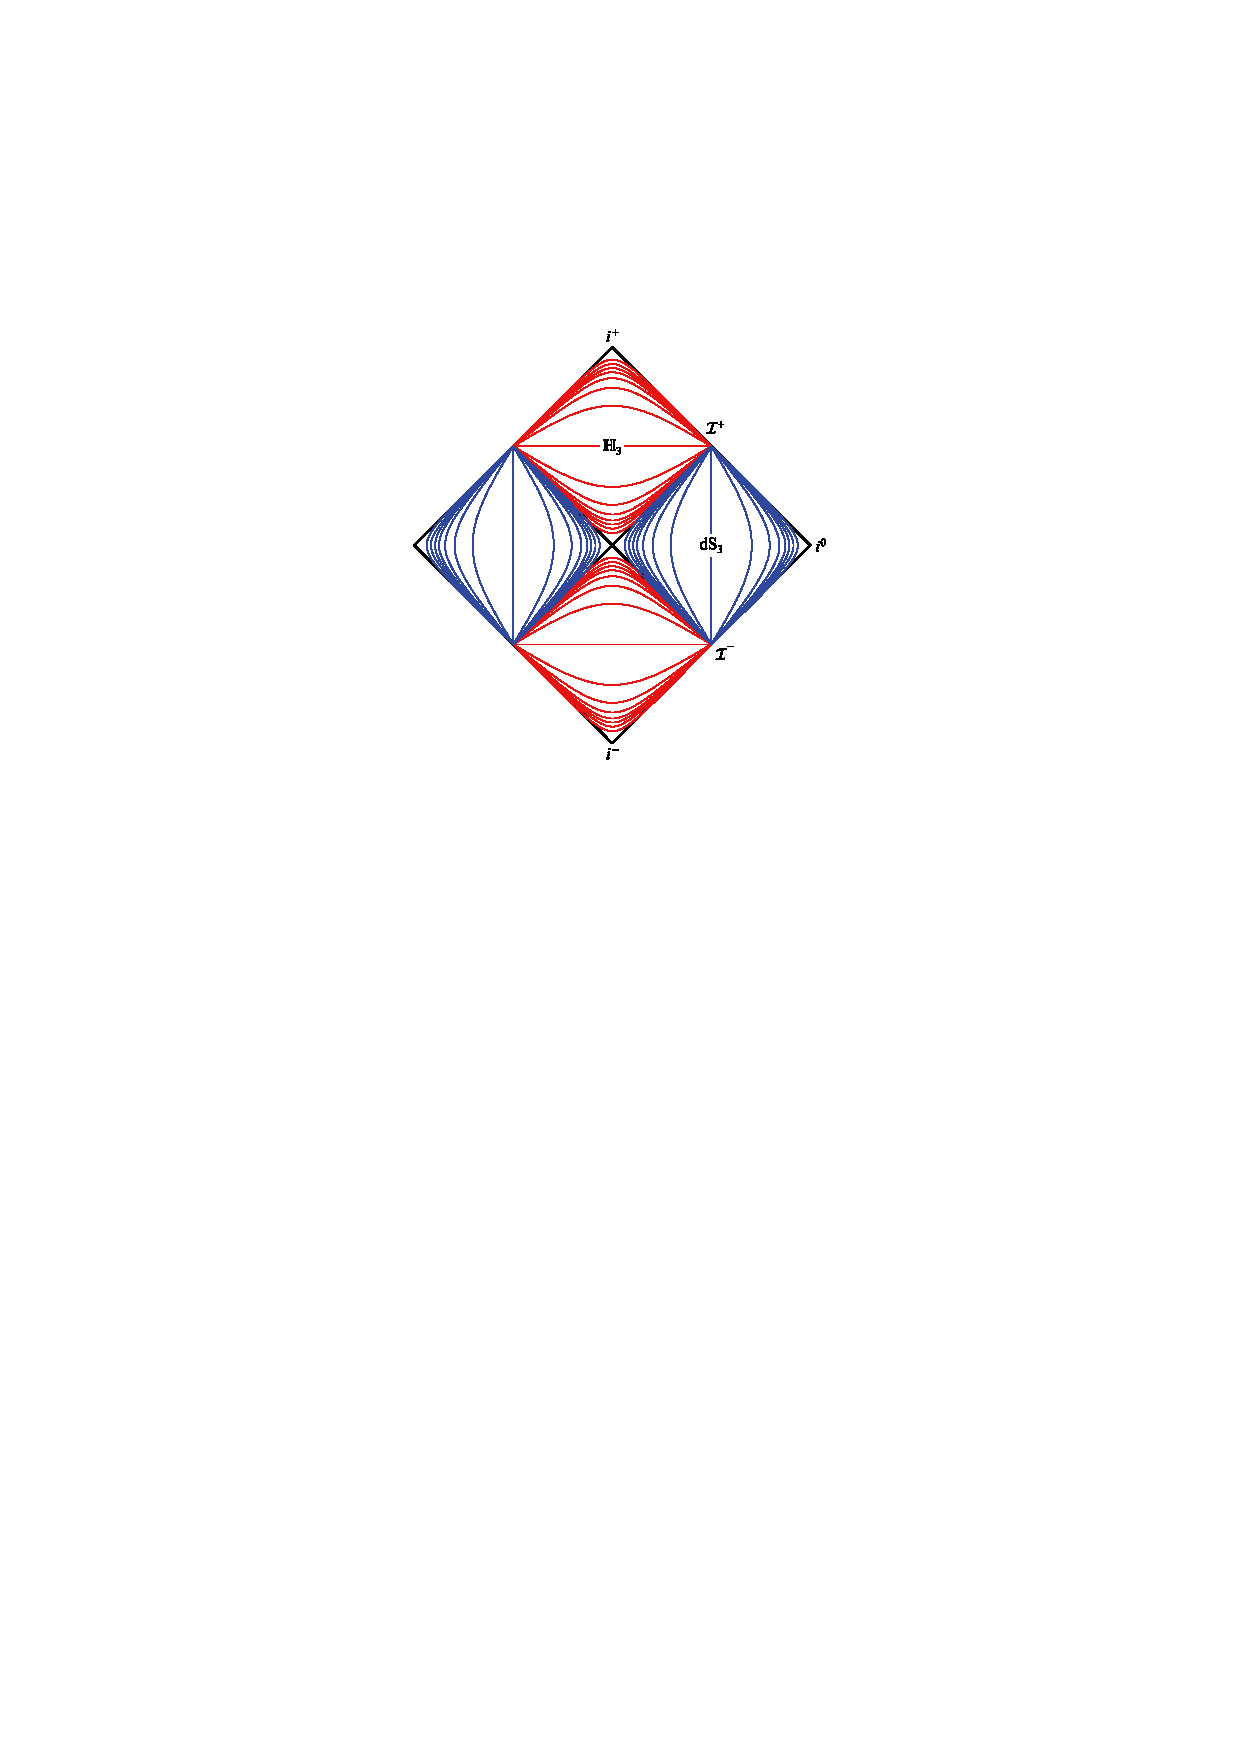
\includegraphics{figs/fig6.pdf}
	\caption{$Mink_4$时空的叶状结构}
	\label{fig:Mink4}
\end{figure}
我们只使用unit的那一层。AdS/CFT对偶里面有一个bulk-to-boundary传播子,在前面的参数化下定义为\cite{Witten:1998qj}:
\begin{equation}
	\boxed{
	G_\Delta(\hat{p};\vec{w})=\left(\frac{y}{y^2+|\vec{z}-\vec{w}|^2}\right)^\Delta =G_\Delta(\hat{p};q)=\frac{1}{(-\hat{p}\cdot q)^\Delta}
	}
\end{equation}
这个传播子在共形变换$q\to q^\prime$,以及所诱导的Lorentz变换$\hat p\to\hat p^\prime$下变换性质为:
\begin{equation}
	G_\Delta(\hat{p'};q')=\left|\frac{\partial\vec{w}'}{\partial\vec{w}}\right|^{-\Delta/d}G_\Delta(\hat{p};q)
\end{equation}
最终的基底肯定是用平面波$\exp\left[\pm im\hat{p}\cdot X\right]$线性组合得到的,这里$+$表示out态,$-$表示in态。而且线性组合要对所有在壳动量构成的平面波求和,所以积分是在$\mathbb{H}_{d+1}$上进行的,积分测度是上面的不变测度:
\begin{equation}
	\int_{\mathbb{H}_{d+1}}[d\hat{p}]\equiv\int_0^\infty\frac{dy}{y^{d+1}}\int d^d\vec{z}=\int_{\hat p^2=-1}\frac{d^{d+1}\hat{p}^i}{\hat{p}^0}
\end{equation}
由于KG方程是一个线性方程,所以线性组合之后的结果都是KG方程的解\sn{只要线性组合的系数与$X$无关就好}。由于$G_\Delta$在共形变换下刚好出来我们需要的共形变换因子,而诱导的Lorentz变换本身不会改变$\hat p \cdot X$和积分测度,所以下面的积分就是满足条件的conformal basis:
\begin{equation}\label{27}
	\boxed{
	\phi_\Delta^\pm(X^\mu;\vec{w})=\int_{\mathbb{H}_{d+1}}[d\hat{p}]G_\Delta(\hat{p};\vec{w})\exp\left[\pm im\hat{p}\cdot X\right]
	}
\end{equation}
注意$\Delta$和$\vec{w}$是用来标记基底的,与$m$无关。但是上面的式子只是形式上的定义,第一不便于计算,第二上式对于$m\in\mathbb{R}_+$是发散的,只有对于$m\in-i{\mathbb{R}_+}$才收敛,所以上式应当看作是先把$m$变成纯虚数积分,然后延拓到实轴。所以考虑直接去找满足条件的KG方程的解,设试探解为:
\begin{equation}
	\phi_\Delta(X^\mu;\vec{w})=\frac{f(X^2)}{(-q\cdot X)^\Delta}
\end{equation}
代入方程得到:
\begin{equation}
	0=4X^2f''(X^2)-2(2\Delta-d-2)f'(X^2)-m^2f(X^2)
\end{equation}
这是虚宗量Bessel方程,考虑$X\to\infty$收敛的解,解正比于第二类修正Bessel函数:
\[f(X^2)\propto\left(\sqrt{-X^2}\right)^{\Delta-\frac{d}{2}}K_{\Delta-\frac{d}{2}}\left(m\sqrt{X^2}\right)\]
前面的比例系数可以从积分表达式\ref{27}积分后最终对比得到:
\begin{equation}
	\phi_\Delta^\pm(X^\mu;\vec{w})=\frac{2^{\frac d2+1}\pi^{\frac d2}}{(im)^{\frac d2}}\frac{(\sqrt{-X^2})^{\Delta-\frac d2}}{(-q(\vec{w})\cdot X\mp i\epsilon)^\Delta}K_{\Delta-\frac d2}(m\sqrt{X^2})
\end{equation}
$\mathcal{A}\equiv\bra{out}\mathcal{S}\ket{\text{in}}$,那么在conformal基底下的散射振幅和原先动量空间散射振幅之间关系为:
\begin{equation}
	\widetilde{\mathcal{A}}(\Delta_i,\vec{w}_i)\equiv\prod_{k=1}^n\int_{\mathbb{H}_{d+1}}[d\hat{p}_k]G_{\Delta_k}(\hat{p}_k;\vec{w}_k)\mathcal{A}(\pm m_i\hat{p}_i^\mu)
\end{equation}
显然其具有CFT中n点关联函数性质:
\begin{equation}
	\widetilde{\mathcal A}(\Delta_{i},\vec{w}_{i}^{\prime}(\vec{w}_{i}))=\prod_{k=1}^{n}\left|\frac{\partial\vec{w}_{k}^{\prime}}{\partial\vec{w}_{k}}\right|^{-\Delta_{k}/d}\widetilde{\mathcal A}(\Delta_{i},\vec{w}_{i})
\end{equation}

前面一直在讲基底,但前面不对$\Delta$进行限制,构造出来的$\{\phi^{\pm}_{\Delta,\vec{w}}\}$极有可能是超完备的。下面我们要干的事情是在构造出来的这些基底里面选某一簇构造正交完备归一基底。

\begin{definition}[shadow transformation]
	对于一个共形维数为$\Delta$的(准)初级场$\mathcal{O}_\Delta(\vec{w})$,其\textbf{shadow}的定义为\cite{Ferrara:1972xe,Ferrara:1972ay,Ferrara:1972uq,Ferrara:1972kab}:
	\begin{equation}
		\begin{aligned}\widetilde{\mathcal{O}}_\Delta(\vec{w})&\equiv\frac{\Gamma(\Delta)}{\pi^{\frac{d}{2}}\Gamma(\Delta-\frac{d}{2})}\int d^d\vec{w}'\frac{1}{|\vec{w}-\vec{w}'|^{2(d-\Delta)}}\mathcal{O}_\Delta(\vec{w}')\end{aligned}
	\end{equation}
	不难发现,场的shadow变成了共形维数为$d-\Delta$的(准)初级场。
\end{definition}
由于$K_\alpha=K_{-\alpha}$,以及下面的恒等式\cite{Simmons-Duffin:2012juh}:
\begin{equation}
	\int d^{d}\vec{z}\frac{1}{|\vec{z}-\vec{w}|^{2(d-\Delta)}}\frac{1}{(-q(\vec{z})\cdot X)^{\Delta}}=\frac{\pi^{\frac{d}{2}}\Gamma(\Delta-\frac{d}{2})}{\Gamma(\Delta)}\frac{(-X^{2})^{\frac{d}{2}-\Delta}}{(-q(\vec{w})\cdot X)^{d-\Delta}}
\end{equation}
得到了一个核心等式:
\begin{equation}\label{eq:27.17}
	\boxed{\widetilde{\phi_\Delta^\pm}(X;\vec{w})=\phi_{d-\Delta}^\pm(X;\vec{w})}
\end{equation}
这实际上直接把空间一分为二,分成某个子空间和它的shadow,我们只用取其中一个构成基就好,因为它的shadow是其线性组合。

在考虑$SO(d+1,1)$的无限维表示\sn{\cite{Sun:2021rrs,Sun:2021thf}这两篇文章比较易读,而且重在比较新,文章\cite{Bissi:2023bhv}的$\S 2.2$是对此内容的一个简短review,更多的阅读材料可以在那里找到。}时会出现所谓\textbf{principal continuous series}的概念:
\begin{equation}
	\boxed{\Delta\in\frac d2+i\mathbb{R}}
\end{equation}
后面构造conformal basis就是用这一series里面的$\Delta$或其子集进行构造,这一点不加证明,后面只是去说明这样确实能得到正确的基底。

首先注意到关于$G_\Delta$的几个正交完备性关系\cite{Costa:2014kfa}:
\begin{equation}
	\int_{-\infty}^{\infty}d\nu\mu(\nu)\int d^{d}\vec{w}G_{\frac{d}{2}+i\nu}(\hat{p}_{1};\vec{w})G_{\frac{d}{2}-i\nu}(\hat{p}_{2};\vec{w})=\delta^{(d+1)}(\hat{p}_{1},\hat{p}_{2})
\end{equation}
这里$\delta$函数是定义在$\mathbb{H}_{d+1}$上也就是$SO(d+1,1)$不变的,积分测度$\mu(\nu)$:
\begin{equation}
	\mu(\nu)=\frac{\Gamma(\frac d2+i\nu)\Gamma(\frac d2-i\nu)}{4\pi^{d+1}\Gamma(i\nu)\Gamma(-i\nu)}
\end{equation}
还有一个
\begin{equation}
	\begin{gathered}
		\int_{H_{d+1}}[d\hat{p}]G_{\frac d2+i\nu}(\hat{p};\vec{w}_{1})G_{\frac d2+i\bar{\nu}}(\hat{p};\vec{w}_{2})= \\
		2\pi^{d+1}\frac{\Gamma(i\nu)\Gamma(-i\nu)}{\Gamma(\frac d2+i\nu)\Gamma(\frac d2-i\nu)}\delta(\nu+\bar{\nu})\delta^{(d)}(\vec{w}_{1}-\vec{w}_{2})+2\pi^{\frac d2+1}\frac{\Gamma(i\nu)}{\Gamma(\frac d2+i\nu)}\delta(\nu-\bar{\nu})\frac{1}{|\vec{w}_{1}-\vec{w}_{2}|^{2(\frac d2+i\nu)}}.
	\end{gathered}
\end{equation}
利用这些关系可以得到\ref{27}的逆变换:
\begin{equation}
	\boxed{e^{\pm im\hat{p}\cdot X}=2\int_0^\infty d\nu\mu(\nu)\int d^d\vec{w}G_{\frac d2-i\nu}(\hat{p};\vec{w})\phi_{\frac d2+i\nu}^\pm(X^\mu;\vec{w})}
\end{equation}
由于平面波基底完备,逆变换的存在性立刻就说明了利用principal continuous series构造出来的$\{\phi^{\pm}_{\Delta,\vec{w}}\}$也完备,而且注意到我们这里利用\ref{eq:27.17}将$\nu$限制在了$\mathbb{R}_+$上,所以:
\begin{equation}\label{eq:27.23}
	\boxed{\Delta\in\frac d2+i\mathbb{R}_{\geq 0}}
\end{equation}
这佐证了前面提到的只需要在空间和其shadow里面取一个就好了。正交性依赖于内积的定义,这里自然的定义KG内积:
\begin{equation}
	(\Phi_1,\Phi_2)=-i\int_\Sigma d^{d+1}X^i\left[\Phi_1(X)\partial_{X^0}\Phi_2^*(X)-\partial_{X^0}\Phi_1(X)\Phi_2^*(X)\right]
\end{equation}
这个定义是Poincar\'e不变的,是与Cauchy面选取无关的。计算得到:
\begin{equation}
	\begin{aligned}
		\left(\phi_{\frac{d}{2}+i\nu_{1}}^{\pm}(X^{\mu};\vec{w_{1}})\right.,&\left.\phi_{\frac{d}{2}+i\nu_{2}}^{\pm}(X^{\mu};\vec{w_{2}})\right) \\
		=&\pm\frac{2^{d+3}\pi^{2d+2}}{m^{d}}\frac{\Gamma(i\nu_{1})\Gamma(-i\nu_{1})}{\Gamma(\frac{d}{2}+i\nu_{1})\Gamma(\frac{d}{2}-i\nu_{1})}\delta(\nu_{1}-\nu_{2})\delta^{(d)}(\vec{w}_{1}-\vec{w}_{2}) \\
		&\pm\cancelto{0}{\frac{2^{d+3}\pi^{\frac{3d}{2}+2}}{m^{d}}\frac{\Gamma(i\nu_{1})}{\Gamma(\frac{d}{2}+i\nu_{1})}\delta(\nu_{1}+\nu_{2})\frac{1}{|\vec{w}_{1}-\vec{w}_{2}|^{2(\frac{d}{2}+i\nu_{1})}}}
	\end{aligned}
\end{equation}
第二项为$0$是因为\ref{eq:27.23}。总结一下,我们得到了$\ket{\text{in}}$和$\ket{\text{out}}$态的基底为:
\begin{equation}
	\boxed{\mathcal{B}^{\pm}=\left\{\begin{array}{c|c}\phi_{\frac{d}{2}+i\nu}^{\pm}(X;\vec{w})&\nu\geq0,\vec{w}\in\mathbb{R}^d\end{array}\right\}}
\end{equation}
它的shadow同样是一组基底:
\begin{equation}
	\boxed{\widetilde{\mathcal{B}}^\pm=\left\{\begin{array}{c|c}\phi_{\frac{d}{2}+i\nu}^\pm(X;\vec{w})&\nu\le0,\vec{w}\in\mathbb{R}^d\end{array}\right\}}
\end{equation}
\subsection{Massless Scalar}
无质量情况看作是有质量情况的极限,作换元$\omega\equiv\frac{m}{2y}$,积分核有如下渐近行为:
\begin{equation}
	G_{\Delta}(y,\vec{z};\vec{w})\xrightarrow{m\to0}\pi^{\frac{d}{2}}\frac{\Gamma(\Delta-\frac{d}{2})}{\Gamma(\Delta)}y^{d-\Delta}\delta^{(d)}(\vec{z}-\vec{w})+\frac{y^{\Delta}}{|\vec{z}-\vec{w}|^{2\Delta}}+\cdots 
\end{equation}
计算得到:
\begin{equation}
	\begin{aligned}\phi_{\frac{d}{2}+i\nu}^{\pm}(X;\vec{w})\xrightarrow{m\to0}&\left(\frac{m}{2}\right)^{-\frac{d}{2}-i\nu}\frac{\pi^{\frac{d}{2}}\Gamma(i\nu)}{\Gamma(\frac{d}{2}+i\nu)}\int_{0}^{\infty}d\omega\omega^{\frac{d}{2}+i\nu-1}e^{\pm i\omega q(\vec{w})\cdot X}\\+&\left(\frac{m}{2}\right)^{-\frac{d}{2}+i\nu}\int d^{d}\vec{z}\frac{1}{|\vec{z}-\vec{w}|^{2(\frac{d}{2}+i\nu)}}\int_{0}^{\infty}d\omega\omega^{\frac{d}{2}-i\nu-1}e^{\pm i\omega q(\vec{z})\cdot X}\end{aligned}
\end{equation}
上面的极限不是well-define的,因为$m^{\pm i\nu}$,但这是个相位,不妨先丢掉,而第二项是第一项的shadow,所以猜测最终应该是下面的形式:\sn{无质量极限下\[\mathbb{H}_3\to\mathcal{I}^\pm: m\hat{p}\to\omega q\]}
\begin{equation}
	\boxed{\varphi_\Delta^\pm(X^\mu;\vec w)\equiv\int_0^\infty d\omega\omega^{\Delta-1}e^{\pm i\omega q\cdot X-\epsilon\omega}=\frac{(\mp i)^\Delta\Gamma(\Delta)}{(-q(\vec w)\cdot X\mp i\epsilon)^\Delta}}
\end{equation}
其中$\Delta\in\mathbb{C}$,需要重新去找寻。这个式子的形式就是所谓\textbf{Mellin变换}\sn{数学上Mellin变换定义为:\[\mathcal{M}(f)(\Delta)=\int_0^\infty d\omega\omega^{\Delta-1}f(\omega)\]其逆变换为:\[f(\omega)=\frac1{2\pi i}\int_{c-i\infty}^{c+i\infty}d\Delta\omega^{-\Delta}\mathcal{M}(f)(\Delta),\]其中$c\in\mathbb{R}$},可以解释成对未来光锥上的某一条射线积分,也就是把所有同“方向”,不同“能量”的平面波组合。注意这个式子有个非常明显的特征,在除去一个归一化因子的意义下,上式结果与$G_\Delta$将$q$替换为$X$得到的结果完全一致。上面变换的逆变换为:
\begin{equation}
	e^{\pm i\omega q\cdot X-\epsilon\omega}=\int_{-\infty}^{\infty}\frac{d\nu}{2\pi}\omega^{-\Delta}\frac{(\mp i)^{\Delta}\Gamma(
		\Delta)}{(-q\cdot X\mp i\epsilon)^{\Delta}},\quad\omega>0,\Re(\Delta)>0
\end{equation}
这说明了$\Re(\Delta)>0$就能保证完备性,而且这组基底张成的空间中很重要的一点是不含零动量的平面波解\sn{这一点是必须的,因为他是KG方程没有物理意义的解,要抛弃掉}。如果选取$\Re(\Delta)=\frac{d}{2}$,$\Im(\Delta)\in\mathbb{R}$,则:
\begin{equation}
	\begin{pmatrix}\varphi_{\frac{d}{2}+i\nu_{1}}^{\pm}(X^{\mu};\vec{w}_{1}),\varphi_{\frac{d}{2}+i\nu_{2}}^{\pm}(X^{\mu};\vec{w}_{2})\end{pmatrix}=\pm8\pi^{d+2}\delta(\nu_{1}-\nu_{2})\delta^{(d)}(\vec{w}_{1}-\vec{w}_{2})
\end{equation}
这个时候注意shadow:
\begin{equation}
	\begin{aligned}
		\widetilde{\varphi_{\frac{d}{2}+i\nu}^{\pm}}(X^{\mu};\vec{w})& =\frac{\Gamma(\frac{d}{2}+i\nu)}{\pi^{\frac{d}{2}}\Gamma(i\nu)}\int d^{d}\vec{z}\frac{1}{|\vec{z}-\vec{w}|^{2(\frac{d}{2}-i\nu)}}\varphi_{\frac{d}{2}+i\nu}^{\pm}(X^{\mu};\vec{z})  \\
		&=(\mp i)^{\frac d2+i\nu}\Gamma(\frac d2+i\nu)\frac{(-X^2)^{-i\nu}}{(-q(\vec{w})\cdot X\mp i\epsilon)^{\frac d2-i\nu}}\\
		\left(\varphi_{\frac{d}{2}+i\nu_1}^{\pm}(X^{\mu};\vec{w_1}),\right.&\left.\widetilde{\varphi_{\frac{d}{2}+i\nu_2}^{\pm}}(X^{\mu};\vec{w_2})\right)=\pm8\pi^{\frac{d}{2}+2}\frac{\Gamma(\frac{d}{2}-i\nu_1)}{\Gamma(-i\nu_1)}\delta(\nu_1-\nu_2)\frac{1}{|\vec{w_1}-\vec{w_2}|^{2(\frac{d}{2}+i\nu_1)}}
	\end{aligned}
\end{equation}
其shadow当然也是一组基底,但并不是$\nu\to-\nu$这么简单了,这导致$\nu$的取值范围也拓宽到了所有实数。总结一下,我们得到了Massless scalar的conformal basis:
\begin{equation}
	\boxed{\mathcal{B}_{m=0}^{\pm}=\left\{\begin{array}{c|c}\varphi_{\frac{d}{2}+i\nu}^{\pm}(X^{\mu};\vec{w})&\nu\in\mathbb{R},\vec{w}\in\mathbb{R}^{d}\end{array}\right\}}
\end{equation}
其shadow也可以作为一组基:
\begin{equation}
	\boxed{\widetilde{\mathcal{B}}_{m=0}^{\pm}=\left\{\begin{array}{c|c}\widetilde{\varphi_{\frac{d}{2}+i\nu}^{\pm}}(X^{\mu};\vec{w})&\nu\in\mathbb{R},\vec{w}\in\mathbb{R}^{d}\end{array}\right\}}
\end{equation}
\begin{remark}
	Mellin变换和傅里叶变换,拉普拉斯变换一样都有卷积定理,它还有个非常重要的\textbf{Ramanujan's Master Theorem}\cite{bougoffa2019note}:
	\begin{theorem}
		若复变函数$f(x)=\sum_{k=0}^\infty\frac{\varphi(k)(-x)^k}{k!}$,则:$$\mathcal{M}_f(x)=\Gamma(s)\mathrm{~}\varphi(-s)$$
	\end{theorem}
	还有一条\textbf{Generalized Ramanujan's Master Theorem}:
	\begin{theorem}
		若复变函数$F(x)=\sum_{k=0}^{\infty}\frac{f^{(k)}\left(0\right)\eta(k)}{k!}x^k$,且$\mathcal{M}(f)(s)=\phi(s)$则:$$\mathcal{M}_F(s)=\phi(s)\eta(-s)$$
	\end{theorem}
	由这一定理可以证明不少积分公式,比如\cite{doi:10.1080/10652469.2014.924114}。
\end{remark}
\subsection{photon \& Graviton}
这两个除了自旋不为0,还有一个比较麻烦的点是需要取定规范。由于自旋不为0,所以基底除了在壳动量、初末态的$\pm$,以及极化矢量带来的$SO(1,d+1)$矢量指标,还需要一个指标用来标记自旋,这里考虑的是无质量玻色子,所以这个指标标记的是粒子的螺旋度,体现为CFT$_d$上的一个$\mathbb{R}^d$张量指标,$a=1,2,\ldots,d$。令在壳动量$k=\omega q$,在Loren规范下可以把平面波基底写为下面的形式:\sn{\[\partial_aq^\mu\equiv\frac{\partial}{\partial w^a}q^\mu(\vec{w})=2(w^a,\delta^{ba},-w^a)\]}:
\begin{equation}
	\partial_aq_\mu e^{\pm i\omega q\cdot X}
\end{equation}
注意Lorenz规范只能将前面的极化矢量确定到一个正比于$k$的项,选取这样的形式相当于完全取定了规范。不难验证$d=2$时,上面的选取就对应\ref{eq:24.7}的选取。
\begin{definition}[Spin\mbox{-}1 Massless Boson, $d\geq 1$]
	~
	\begin{itemize}
		\item 在壳:\footnote{满足的是Proca方程}
		\begin{equation}
			\left(\frac{\partial}{\partial X^\sigma}\frac{\partial}{\partial X_\sigma}\delta_\nu^\mu-\frac{\partial}{\partial X^\nu}\frac{\partial}{\partial X_\mu}\right)A_{\mu a}^{\Delta\pm}(X^\rho;\vec{w})=0
		\end{equation}
		\item 协变:
		\begin{equation}
			A_{\mu a}^{\Delta\pm}\left(\Lambda^{\rho}{}_{\nu}X^{\nu};\vec{w}'(\vec{w})\right)=\frac{\partial w^{b}}{\partial{w'^{a}}}\left|\frac{\partial\vec{w}'}{\partial\vec{w}}\right|^{-(\Delta-1)/d}\Lambda_{\mu}{}^{\sigma}A_{\sigma b}^{\Delta\pm}(X^{\rho};\vec{w})
		\end{equation}
	\end{itemize}
\end{definition}
$\mathbb{H}_{d+1}$上面的 Spin\mbox{-}1 bulk-to boundary 传播子为$G^\Delta_{\mu;q}$\sn{后面只要是$a,b,c$指标就是$\mathbb{R}^d$上的,在只要是$\mu,\nu,\sigma$指标就是$\mathbb{R}^{1,d+1}$上的},计算上更常用的是其 \textbf{uplift} $G^\Delta_{\mu;\nu}$,定义为:\sn{其实就是拉回映射}
\begin{equation}
	G^\Delta_{\mu;q}=\frac{\partial q^\nu}{\partial w^a}G_{\mu;\nu}^\Delta(\hat{p};q)
\end{equation}
\begin{equation}
	G_{\mu;\nu}^{\Delta}(\hat{p};q)=\frac{(-q\cdot\hat{p})\eta_{\mu\nu}+q_{\mu}\hat{p}_{\nu}}{(-q\cdot\hat{p})^{\Delta+1}}
\end{equation}
uplift之后,$G^\Delta_{\mu;\nu}$就是一个标量CFT$_d$,而且是$\mathbb{R}^{1,d+1}$上的2\mbox{-}tensor:
\begin{equation}
	G_{\mu;\nu}^{\Delta}(\Lambda\hat{p};\Lambda q)=\left|\frac{\partial\vec{w}'}{\partial\vec{w}}\right|^{-\Delta/d}\Lambda^{\rho}{}_{\mu}\Lambda^{\sigma}{}_{\nu}G^{\Delta}{}_{\rho;\sigma}(\hat{p};q)
\end{equation}
而且关于两个自变量还满足横向条件:
\begin{equation}\label{eq:t}
	\hat{p}^{\mu}G_{\mu;\nu}^{\Delta}(\hat{p};q)=0,\quad q^{\nu}G_{\mu;\nu}^{\Delta}(\hat{p};q)=0
\end{equation}
根据前面的标量场经验,不难猜测$A$的形式就是$G$把$q$换成$X$:
\begin{equation}
	\boxed{
		\begin{aligned}
			A_{\mu a}^{\Delta,\pm}(X^{\mu};\vec{w})& {=\frac{\partial_{a}q_{\mu}}{(-q\cdot X\mp i\epsilon)^{\Delta}}+\frac{\partial_{a}q\cdot X}{(-q\cdot X\mp i\epsilon)^{\Delta+1}}q_{\mu}} \\
			&=-\frac{1}{(-q\cdot X\mp i\epsilon)^{\Delta-1}}\frac{\partial}{\partial X^{\mu}}\frac{\partial}{\partial w^{a}}\log(-q\cdot X\mp i\epsilon)
		\end{aligned}
	}
\end{equation}
证明略。下面计算其shadow。
\begin{definition}[shadow for spinning fields]
	对于自旋为$J$的场,其会导致带有$J$个$\mathbb{R}^d$上的指标$a_1,\ldots,a_J$,而且这些指标是无迹且全对称的,或者说$\mathcal{O}^\Delta_{a_1\cdot\cdot\cdot a_J}(\vec{w})$是$SO(d)$的无迹对称张量表示,即Spin\mbox{-}J表示。计算其shadow最简单的方式是使用其uplift计算,然后再投影回来,uplift与其自身的关系为:
	\begin{equation}
		\mathcal{O}^\Delta_{a_1\cdots a_J}(\vec{w})=\frac{\partial q^{\mu_1}}{\partial w^{a_1}}\cdots\frac{\partial q^{\mu_J}}{\partial w^{a_J}}\mathcal{O}^\Delta_{\mu_1\cdots\mu_J}(\vec{w})
	\end{equation}
	uplift与其自变量之间存在类似\ref{eq:t}的横向关系。
	\begin{equation}
		\boxed{
		\widetilde{\mathcal{O}^\Delta}_{\mu_1\cdots\mu_J}(\vec{w})=\frac{\Gamma(\Delta+J)}{\pi^{\frac d2}(\Delta-1)_J\Gamma(\Delta-\frac d2)}\int d^d\vec{w}^{\prime}\frac{\prod_{n=1}^J\left[\delta_{\mu_n}^{\nu_n}(-\frac12q\cdot q^{\prime})+\frac12q_{\mu_n}^{\prime}q^{\nu_n}\right]}{(-\frac12q\cdot q^{\prime})^{d-\Delta+J}}\mathcal{O}^\Delta_{\nu_1\cdots\nu_J}(\vec{w}^{\prime})}
	\end{equation}
	这里$(a)_{J}\equiv\Gamma(a+J)/\Gamma(a)$,称为Pochhammer符号,而且不难发现上面的定义对于某些$\Delta$不是well-define的,所以需要解析延拓到全部复平面。
\end{definition}
利用上面定义计算得到:
\begin{equation}
	\boxed{
	\widetilde{A_{\mu a}^{\Delta,\pm}}(X^\mu;\vec{w})=(-X^2)^{\frac{d}{2}-\Delta}A_{\mu a}^{d-\Delta,\pm}(X^\mu;\vec{w})
	}
\end{equation}
和无质量标量场一样,不是正比于$A_{\mu a}^{d-\Delta,\pm}$。现在还没有讨论我们的计算是在哪个规范下进行的,但其实前面对$A_{\mu a}^{\Delta,\pm}$那些在壳协变的要求就已经为我们完全取定了规范,是Lorenz和radial规范同时加上去:\sn{这两个规范是可以同时取的,见\cite{PhysRevD.76.084013}}
\begin{equation}
	X^{\mu}A_{\mu a}^{\Delta,\pm}(X^{\mu};\vec{w})=0,\quad\partial^{\mu}A_{\mu a}^{\Delta,\pm}(X^{\mu};\vec{w})=0.
\end{equation}
下表总结了$A_{\mu a}^{\Delta,\pm}$及其 shadow 为 pure gauge\sn{pure gauge就是说可以从$A=0$通过规范变换变过来,所以场强张量为0,$A$可以写为$\frac{i}{g}U\partial_\mu U^\dagger$的形式}的条件:
\begin{center}
	\begin{tabular}[H]{|c|c|c|}
		\hline & $d=2$ & $d \neq 2$ \\
		\hline$A_{\mu a}^{\Delta, \pm}$ & & $\Delta=1$ \\
		& $\Delta=1$ & \\
		$\widetilde{A_{\mu a}^{d-\Delta, \pm}}$& & $\times$ \\
		\hline
	\end{tabular}
\end{center}
回顾一些前面给的平面波基底是在Lorenz规范下给的,不一定满足radial规范,所以$A$不能写成平面波基底的积分变换形式,但是:
\begin{equation}
	\boxed{
	\varphi_{\mu a}^{\Delta,\pm}(X^{\mu};\vec{w})=\int_0^\infty d\omega\omega^{\Delta-1}\left(\partial_aq_\mu e^{\pm i\omega q\cdot X-\epsilon\omega}\right)=(\mp i)^\Delta\Gamma(\Delta)\frac{\partial_aq_\mu}{(-q\cdot X\mp i\epsilon)^\Delta}
	}
\end{equation}
和$A_{\mu a}^{\Delta,\pm}$之间只差一个规范变换\sn{$\frac{\partial}{\partial X^\mu}\left(\frac{\partial_aq\cdot X}{(-q\cdot X\mp i\epsilon)^\Delta}\right)$},那么在计算散射振幅这种与规范选取无关的物理量的时候,用两组基底都能得到同样的结果,但是注意用$\varphi_{\mu a}^{\Delta,\pm}$做基底的时候就没有协变的条件了,但是好处在两基底振幅之间是Mellin变换的形式。在下面的内积定义下:
\begin{equation}
	(A_{\mu},A'_{\mu'})=-i\int _\Sigma d^{d+1}X^i\left[A^{\rho}F'^*_{0\rho}-A'^{\rho*}F_{0\rho}\right]
\end{equation}
当选取$\boxed{\Delta\in\frac{d}{2}+\mathrm{i}\mathbb{R}}$时构成完备基底,其shadow亦然。

这组基底虽说是photon的,但实际上非阿贝尔情形也完全适用,因为每个色指标的场满足相同的方程,相同的协变条件,所以上面的推导完全不变,这是很容易接受的,因为平面波基底对于photon和gluon都是一样通用的。

现在来看引力子的情况,首先在Lorenz\sn{$\partial^{\mu}h_{\mu\nu}-\frac12\partial_{\nu}h^{\rho}{}_{\rho}=0,$}、无迹规范下平面波基底可以写为:
\begin{equation}
	g_{\mu\nu;a_1a_2}^{\pm}(X;\omega,q)=P_{a_1a_2}^{b_1b_2}\partial_{b_1}q_\mu\partial_{b_2}q_\nu e^{\pm i\omega q\cdot X}
\end{equation}
这里:
\begin{equation}
	P_{a_1a_2}^{b_1b_2}\equiv\delta_{(a_1}^{b_1}\delta_{a_2)}^{b_2}-\frac{1}{d}\delta_{a_1a_2}\delta^{b_1b_2}
\end{equation}
\begin{definition}[Graviton, $d\geq 2$]
	~
	\begin{itemize}
		\item 指标约束:
		\begin{equation}
			\begin{array}{l}h_{\mu_1\mu_2;a_1a_2}^{\Delta,\pm}=h_{\mu_2\mu_1;a_1a_2}^{\Delta,\pm},\\h_{\mu_1\mu_2;a_1a_2}^{\Delta,\pm}=h_{\mu_1\mu_2;a_2a_1}^{\Delta,\pm},\quad\delta^{a_1a_2}h_{\mu_1\mu_2;a_1a_2}^{\Delta,\pm}=0\end{array}
		\end{equation}
		第一个约束是几何上要求度规对称,第二个是要求$\mathbb{R}^d$指标无迹且对称。
		\item 在壳:\footnote{满足的是Linearized Einstein方程}
		\begin{equation}
			\partial_\sigma\partial_\nu {h^\sigma}_{\mu;a_1a_2}+\partial_\sigma\partial_\mu {h^\sigma}_{\nu;a_1a_2}-\partial_\mu\partial_\nu {h^\sigma}_{\sigma;a_1a_2}-\partial^\rho\partial_\rho h_{\mu\nu;a_1a_2}=0
		\end{equation}
		\item 协变:
		\begin{equation}
			h_{\mu_1\mu_2;a_1a_2}^{\Delta,\pm}\left(\Lambda_{\nu}^{\rho}X^{\nu};\vec{w}'(\vec{w})\right)=\frac{\partial w^{b_1}}{\partial w'^{a_1}}\frac{\partial w^{b_2}}{\partial w'^{a_2}}\left|\frac{\partial\vec{w'}}{\partial\vec{w}}\right|^{-(\Delta-2)/d}\Lambda_{\mu_1}^{\sigma_1}\Lambda_{\mu_2}^{\sigma_2}h_{\sigma_1\sigma_2;b_1b_2}^{\Delta,\pm}(X^\rho;\vec{w})
		\end{equation}
	\end{itemize}
\end{definition}
利用$\mathbb{H}_{d+1}$上面的 Spin\mbox{-}2 bulk-to boundary 传播子:
\begin{equation}\label{eq:27.55}
	\boxed{
		\begin{aligned}
			h_{\mu_1\mu_2;a_1a_2}^{\Delta,\pm}(X;\vec{w})&=P_{a_1a_2}^{b_1b_2}\frac{\left[(-q\cdot X)\partial_{b_1}q_{\mu_1}+(\partial_{b_1}q\cdot X)q_{\mu_1}\right]\left[(-q\cdot X)\partial_{b_2}q_{\mu_2}+(\partial_{b_2}q\cdot X)q_{\mu_2}\right]}{(-q\cdot X)^{\Delta+2}}\\
			&=P_{a_{1}a_{2}}^{b_{1}b_{2}}\frac{1}{(-q\cdot X\mp i\epsilon)^{\Delta-2}}\partial_{b_{1}}\partial_{\mu_{1}}\log(-q\cdot X\mp i\epsilon)\partial_{b_{2}}\partial_{\mu_{2}}\log(-q\cdot X\mp i\epsilon)
		\end{aligned}
		}
\end{equation}
其shadow:
\begin{equation}
	\widetilde {h_{\mu_1\mu_2;a_1a_2}^{\Delta,\pm}}(X;\vec{w})=(-X^2)^{\frac{d}{2}-\Delta}h_{\mu_1\mu_2;a_1a_2}^{d-\Delta,\pm}(X;\vec{w})
\end{equation}
前面实际上选取了规范:
\begin{equation}
	\eta^{\mu_1\mu_2}h_{\mu_1\mu_2;a_1a_2}^{\Delta,\pm}=0,\quad\partial^{\mu}h_{\mu\mu_2;a_1a_2}^{\Delta,\pm}=0,\quad X^{\mu}h_{\mu\mu_2;a_1a_2}^{\Delta,\pm}=0
\end{equation}
有Pure gauge条件:\sn{可以写为$\partial_{(\mu}\xi_{\nu)}$的形式}
\begin{center}
	\begin{tabular}[H]{|c|cc|c|}
		\hline & \multicolumn{2}{c|}{$d=2$} & $d \geq 2$ \\
		\hline$h_{\mu_1\mu_2;a_1a_2}^{\Delta,\pm}$ & &$\Delta=0$& $\Delta=0,1$ \\
		& $\Delta=1$ & & \\
		$\widetilde{h_{\mu_1\mu_2;a_1a_2}^{d-\Delta,\pm}}$& &$\Delta=2$ & $\times$ \\
		\hline
	\end{tabular}
\end{center}
同样,前面的平面波基底不满足radial规范,但利用Mellin变换后得到的:
\begin{equation}
	\boxed{
	\begin{aligned}
		\varphi_{\mu_1\mu_2;a_1a_2}^{\Delta,\pm}(X^\mu;\vec{w})&=\int_0^\infty d\omega\omega^{\Delta-1}g_{\mu_1\mu_2;a_1a_2}^{\Delta,\pm}(X^\mu;\omega,q^\mu)\\&=(\mp i)^\Delta\Gamma(\Delta)P_{a_1a_2}^{b_1b_2}\frac{\partial_{b_1}q_{\mu_1}\partial_{b_2}q_{\mu_2}}{(-q\cdot X\mp i\epsilon)^\Delta}
	\end{aligned}
}
\end{equation}
与\ref{eq:27.55}只差一个规范变换\begin{margintable}\footnotesize 
	\begin{tabularx}{\marginparwidth}{|X}
		Because:
		\[\frac{\partial_bq_{(\mu_1}q_{\mu_2)}}{(-q\cdot X)^\Delta}=\frac{\partial_{(\mu_1}}{\Delta-1}\left(\frac{\partial_bq_{\mu_2)}}{(-q\cdot X)^{\Delta-1}}\right)\]
		\[\frac{q_{\mu_1}q_{\mu_2}}{(-q\cdot X)^\Delta}=\frac{\partial_{(\mu_1}}{\Delta-1}\left(\frac{q_{\mu_2)}}{(-q\cdot X)^{\Delta-1}}\right)\]
	\end{tabularx}
\end{margintable}。在下面的内积意义下:
\begin{equation}
	\begin{aligned}
		(h_{\mu\nu},h_{\mu^{\prime}\nu^{\prime}}^{\prime})& =-i\int d^{d+1}X^{i}\Big[h^{\mu\nu}\partial_{0}{h^{\prime}}_{\mu\nu}^{*}-2h^{\mu\nu}\partial_{\mu}{h^{\prime}}_{0\nu}^{*}+h\partial^{\mu}{h^{\prime}}_{0\mu}^{*}-h\partial_{0}{h^{\prime}}^{*}+h_{0\mu}{\partial^{\mu}{h^{\prime}}^{*}}  \\
		&-(h\leftrightarrow{h^{\prime}}^{*})\Big]
	\end{aligned}
\end{equation}
$\boxed{\Delta\in\frac{d}{2}+\mathrm{i}\mathbb{R}}$时构成完备基底,其shadow亦然。
\begin{remark}
	$SO(1,d+1)$群的无限维不可约幺正表示由共形维数$\Delta\in\mathbb{C}$和$SO(d)$的表示去标记(或者说取决于对应的$SO(d)$是哪个自旋表示)。前面找的基底就是在找表示,$\Delta$和$J$之间是有约束的,具体来说有下面几个Series:
	\begin{itemize}
		\item Principal Series $\mathcal{P}$: $\forall J\in\mathbb{N},\quad \Delta\in\frac{d}{2}+\mathrm{i}\mathbb{R}$
		\item Complementary Series $\mathcal{C}$: $\Delta=\frac{d}{2}+c$,其中$J=0$时$0<|c|\leq\frac{d}{2}$,$J\geq 1$时$0<|c|\leq\frac{d}{2}-1$
		\item Discrete Series $\mathcal{D}$: 对于奇数维数$d$,任意$J$,$\Delta$可取半整数或者整数
	\end{itemize}
	表示$[\Delta,J]$的shadow就是表示$[d-\Delta,J]$,这两个表示是等价表示。
\end{remark}
\subsection{Restrict to Mink$_{4}$}
根据前面的一系列一般性讨论,回到Mink$_{4}$情况很简单,这里只是用文献中比较常用的记号重新写一遍。\sn{\cite{Donnay:2020guq}$\S 2$基本上是很好的总结}

标量场:
\begin{equation}
	\phi_{\Delta,m}\left(\Lambda^{\mu}{}_{\nu}X^{\nu};\frac{aw+b}{cw+d},\frac{\bar{a}\bar{w}+\bar{b}}{\bar{c}\bar{w}+\bar{d}}\right)=|cw+d|^{2\Delta}\phi_{\Delta,m}(X^{\mu};w,\bar{w})
\end{equation}

无质量规范玻色子:
\begin{equation}
	A_{\mu;a}^{\Delta,\pm}\left({\Lambda^{\rho}}_{\nu}X^{\nu};\frac{aw+b}{cw+d},\frac{\bar{a}\bar{w}+\bar{b}}{\bar{c}\bar{w}+\bar{d}}\right)=(cw+d)^{2h}(\bar{c}\bar{w}+\bar{d})^{2\bar{h}}{\Lambda_{\mu}}^{\sigma}A_{\sigma;a}^{\Delta,\pm}(X^{\rho};w,\bar{w})
\end{equation}
无质量规范玻色子只有两种螺旋度选取,对应这里$a=w,\bar w$,分别有$J=+1,-1$。

引力子:
\begin{equation}
	h_{\mu\nu;a}^{\Delta,\pm}\left(\Lambda^{\mu}{}_{\nu}X^{\nu};\frac{aw+b}{cw+d},\frac{\bar{a}\bar{w}+\bar{b}}{\bar{c}\bar{w}+\bar{d}}\right)=(cw+d)^{\Delta+J}(\bar{c}\bar{w}+\bar{d})^{\Delta-J}{\Lambda_{\mu}}^{\rho}{\Lambda_{\nu}}^{\sigma}h_{\rho\sigma,a}^{\Delta,\pm}(X^{\mu};w,\bar{w})
\end{equation}
同样的引力子也只有两种螺旋度选取,对应$a=ww,\bar w\bar w$,分别对应$J=+2,-2$。
不难看出这些情况共形权$(h,\bar h)=\frac12(\Delta+J,\Delta-J)$,$h-\bar h$确实就对应自旋。后面考虑有质量玻色子这里的$J$的取值范围就会从$-s\sim s$。

\subsection{Conformally Soft photon \& Graviton}
前面的基底其实对于软光子和软引力子要进行修正,文献\cite{Donnay:2018neh}首先进行了分析,文献\cite{Donnay:2020guq}给出了更一般的处理技术,并进行了推广,文献\cite{Pano:2021ewd}又对费米子情况进行了讨论\sn{本笔记不涉及这部分内容}。
\subsubsection{Photon}
处理soft sector最naive的想法就是直接取$\Delta=1$得到对应的一个零模解:
\begin{equation}
	A_{\mu;a}^\mathrm{G}\equiv\lim_{\Delta\to1}A_{\mu;a}^{\Delta,\pm}=\partial_{\mu}\alpha_{a}^1,\quad\alpha_a^1=-\frac{\partial_aq\cdot X}{a\cdot X}
\end{equation}
这个解真正对应对称性自发破缺后产生的软光子,所以我们成为Goldstone mode。注意由于能量趋于0,正负能解,也就是出入射解简并了,正是这种简并暗示为了构造完备的基底,我们还需要找到另一个与其线性无关的零模\sn{文献中常称为Canonical Partner}。不难验证下面的波函数也满足Proca方程:
\begin{equation}
	A_{\mu;a}^{\mathrm{log,}\pm}\equiv\lim_{\Delta\to1}\partial_\Delta\left(A_{\mu;a}^{\Delta,\pm}+\widetilde{A_{\mu;a}^{\Delta,\pm}}\right)\xrightarrow{\text{regularize}}-\log\left[-X^2\mp2i\varepsilon X^0-\varepsilon^2\right]\partial_\mu\left(\frac{\partial_a(q\cdot X\pm i\varepsilon q^0)}{-q\cdot X\mp i\varepsilon q^0}\right)
\end{equation}
而且也是$\Delta=1$的Primary wavefunction。对应可以构建场强张量为:
\begin{equation}
	F_{\mu\nu;a}^{\mathrm{log},\pm}=-\frac{2(X_\mu\pm i\varepsilon\delta_\mu^0)}{X^2\pm2i\varepsilon X^0+\varepsilon^2}\partial_\nu\left(\frac{\partial_a(q\cdot X\pm i\varepsilon q^0)}{-q\cdot X\mp i\varepsilon q^0}\right)-(\mu\leftrightarrow\nu)
\end{equation}
我们感兴趣的是下面的组合:\footnote{计算中用到了下面的常见等式:\[\begin{aligned}
		&\begin{aligned}\delta(x)&=-\frac{1}{2\pi i}\left(\frac{1}{x+i\varepsilon}-\frac{1}{x-i\varepsilon}\right),\end{aligned} \\
		&\begin{aligned}\delta'(x)&=\frac{1}{2\pi i}\left(\frac{1}{(x+i\varepsilon)^2}-\frac{1}{(x-i\varepsilon)^2}\right)=-\frac{\delta(x)}{x}\end{aligned}
	\end{aligned}\]}
\begin{equation}
	F_{\mu\nu;a}^\mathrm{CS}\equiv\frac1{2\pi i}\left(F_{\mu\nu;a}^{\log,+}-F_{\mu\nu;a}^{\log,-}\right)=2X_{\mu}A_{\nu;a}^\mathrm{G}\left(\delta\left(X^2\right)+\frac{(q\cdot X)}{X^2}\delta(q\cdot X)\right)-(\mu\leftrightarrow\nu)
\end{equation}
对应的规范场为:
\begin{equation}
	A_{\mu;a}^\mathrm{CS}=(q\cdot X)\log[X^2]A_{\mu;a}^\mathrm{G}\delta(q\cdot X)+A_{\mu;a}^\mathrm{G}\Theta\left(X^2\right)
\end{equation}
这个就是所谓的\textbf{Conformally Soft Gauge Field},仍旧是满足场方程且$\Delta=1$的初级场。可以验证G和CS模式是互相正交的:\sn{这里用全纯或者反全纯的下标表示$\pm 1$的螺旋度。}
\begin{equation}
	i(A_w^\mathrm{CS}(w),A_{w^{\prime}}^\mathrm{G}(w^{\prime}))_{\mathcal{I}^+}=8\pi^2\delta^{(2)}(w-w^{\prime})
\end{equation}
所以G,CS和其他$\operatorname{Im}(\Delta)\neq 0$的谱一起构成了完备正交基底。其进一步的物理意义待到和天球上的Ka\v{c}-Moody流一起讲。
\subsubsection{Graviton}
考虑引力子的思路和光子几乎是一样的,尽管前面给出引力子Pure gauge条件时除了$\Delta=1$,还有$\Delta=0,2$,但是单单从实用角度上看我们不必分析$\Delta=0,2$,因为只需要$\operatorname{Re}(\Delta)=1$的基底就能构成完备基了,出于物理意义上可能会稍加讨论。

首先依旧是naive的Goldstone mode:
\begin{equation}
	h_{\mu\nu;a}^\mathrm{G}\equiv\lim_{\Delta\to1}h_{\mu\nu;a}^{\Delta,\pm}=\partial_\mu\xi_{\nu;a}+\partial_\nu\xi_{\mu;a},\quad\xi_{\mu;a}\equiv-\frac18\partial_a^2[q_\mu\log(-q\cdot X)]
\end{equation}
然后是$\log$部分:
\begin{equation}
	h_{\mu\nu;a}^{\mathrm{log},\pm}\equiv\lim_{\Delta\to1}\partial_\Delta\left(h_{\mu\nu;a}^{\Delta,\pm}+\widetilde{h_{\mu\nu;a}^{\Delta,\pm}}\right)
\end{equation}
正规化,找场强,线性组合$\log$部分,所有的这些后续计算都和光子的方法是一致的,最终结果为:
\begin{equation}
	h_{\mu\nu;a}^\mathrm{ST}=(q\cdot X)\log[X^2]h_{\mu\nu;a}^\mathrm{G}\delta(q\cdot X)+h_{\mu\nu;a}^\mathrm{G}\Theta\left(X^2\right)
\end{equation}
这满足场方程,且$\Delta=1$,由于这个模式与某个Supertranslation对应,所以我们叫ST mode,而没有用conformally soft graviton这个名称。同样可以证明G和ST是相互正交的:
\begin{equation}
	(h_{ww}^\mathrm{ST}(w),h_{w'w'}^\mathrm{G}(w'))_{\mathcal{I}^+}=\frac{i\pi^2}2\gamma_{w\bar{w}}\delta^{(2)}(w-w')
\end{equation}
\begin{remark}
	计算中用到了一个之后可能会用到的技术,这来源于文献\cite{Dolan:2011dv},一般维数看古老文献\cite{Symanzik:1972wj}。定义下面的Conformal Integrals(2D):
	\begin{equation}
		I_n=\frac1{2\pi}\int d^2z\prod_{i=1}^n\frac1{(z-z_i)^{h_i}}\frac1{(\bar{z}-\bar{z}_i)^{\bar{h}_i}}
	\end{equation}
	其中:
	$$
		\sum_{i=1}^nh_i=\sum_{i=1}^n\bar{h}_i=2,h_i-\bar{h}_i\in\mathbb{Z}
	$$
	第一个等式确保了在$SL(2,\mathbb{C})$下积分是共形协变的,第二个条件确保了积分单值性。正是由于与共形变换之间的密切联系,让这个看似非常难以计算的积分可以被极大的限制住,$n=2$的情况为:
	\begin{equation}
		I_2=\frac{\Gamma(1-h_1)\Gamma(1-h_2)}{\Gamma(\bar{h}_1)\Gamma(\bar{h}_2)}(-1)^{h_1-\bar{h}_1}2\pi\delta^{(2)}(z_1-z_2)
	\end{equation}
	$n=3,4$的情况请见文献中的讨论。
\end{remark}
下面来考虑$\Delta=2$的Goldstone模式:
\begin{equation}
	\widetilde{h_{\mu\nu;a}^{\Delta=2}}\equiv-X^2h_{\mu\nu;a}^{\Delta=2}=\partial_\mu\zeta_{\nu;a}+\partial_\nu\zeta_{\mu;a}
\end{equation}
其中Pure Gauge:
\begin{equation}
	\zeta_{\mu;a}\equiv-\frac1{24}\partial_a^3[X^\rho(q_\rho\partial_{\bar{a}}q_\mu-q_\mu\partial_{\bar{a}}q_\rho)\mathrm{log}(-q\cdot X)]
\end{equation}
把度规$h$在Bondi坐标下写出啦,就可以找到对应的Bondi News:
\begin{equation}
	\widetilde{N}_{zz;ww}^{\Delta=2}=\frac1{(z-w)^4}=D_z^3Y^z_{ww},\quad Y_{ww}^z\equiv-\frac1{6(z-w)}
\end{equation}
后面会看到它与CCFT上能动张量之间的联系。
\subsection{Massive Bosons}
文献\cite{Law:2020tsg}率先给出了有质量玻色子的分析。而且利用这一基底计算了一些振幅。为了总结结论,首先要介绍\cite{Costa:2011mg}中的Polynomial Encoding。
\subsubsection{Polynomial encoding of symmetric traceless transverse tensors}
对于$\mathbb{H}_3$上定义的任意一个spin\mbox{-s}的对称无迹transverse张量$H_{\mu_1\cdot\cdot\cdot\mu_s}(\hat{p})$,可以在下面的辅助矢量定义的子流形上:
\[\hat{p}^2+1=Y^2=\hat{p}\cdot Y=0\]
将张量编码进在此子流形上定义的多项式上:\sn{后面对此多项式的一切操作都要记得是在这个子流形上完成的}
\begin{equation}
	H(\hat{p},Y)=H_{\mu_1\cdot\cdot\cdot\mu_s}(\hat{p})Y^{\mu_1}\cdotp\cdotp\cdotp Y^{\mu_s}
\end{equation}
利用下面定义的微分算符:\sn{\[K_{\mu}K_{\nu}=K_{\nu}K_{\mu},\hat{p}^{\mu}K_{\mu}=0,K_{\mu}K^{\mu}=0\]}
\begin{equation}
	\begin{aligned}
		K_{\mu}=& \begin{aligned}\frac{1}{2}\left(\frac{\partial}{\partial Y^{\mu}}+\hat{p}_{\mu}\left(\hat{p}\cdot\frac{\partial}{\partial Y}\right)\right)+\left(Y\cdot\frac{\partial}{\partial Y}\right)\frac{\partial}{\partial Y^{\mu}}\end{aligned}  \\
		&+\hat{p}_{\mu}\left(Y\cdot\frac{\partial}{\partial Y}\right)\left(\hat{p}\cdot\frac{\partial}{\partial Y}\right)-\frac{Y_{\mu}}{2}\left(\frac{\partial^{2}}{\partial Y\cdot\partial Y}+\left(\hat{p}\cdot\frac{\partial}{\partial Y}\right)\left(\hat{p}\cdot\frac{\partial}{\partial Y}\right)\right)
	\end{aligned}
\end{equation}
可以将多项式还原成张量本身:\sn{有点像配分函数,这里$(\cdot)_s$是Pochhammer符号}
\begin{equation}
	H_{\mu_1\cdots\mu_s}(\hat{p})=\frac{1}{s!\left(\frac{1}{2}\right)_s}K_{\mu_1}\cdotp\cdotp\cdotp K_{\mu_s}H(\hat{p},Y)
\end{equation}
对$\hat p$的协变导数定义为:\sn{满足$Y\cdot\nabla_{\hat{p}}=Y\cdot\partial_{\hat{p}}$}
\begin{equation}
	\nabla_{\hat{p}^{\mu}}=\frac{\partial}{\partial\hat{p}^{\mu}}+\hat{p}_{\mu}\left(\hat{p}\cdot\frac{\partial}{\partial\hat{p}}\right)+Y_{\mu}\left(\hat{p}\cdot\frac{\partial}{\partial Y}\right)
\end{equation}
下面考虑光锥(正则部分)上面的spin\mbox{-}J的对称无迹transverse张量$F_{\mu_{1}\cdots\mu_{J}}(q)$,可以把它看作是天球上的spin\mbox{-}J 对称无迹张量$f_{a_{1}\cdots a_{J}}(w,\bar{w})$的uplift。对称无迹已经把$f$限制成只有两个不为$0$的分量了:\sn{In general $\tilde{f}_J\neq f_J^*$}
\begin{equation}
	f_J(w,\bar{w})=f_{w\cdots w}(w,\bar{w})\quad\mathrm{~and~}\quad\tilde{f}_J(w,\bar{w})=f_{\bar{w}\cdots\bar{w}}(w,\bar{w})
\end{equation} 
所以
\begin{equation}\label{eq:27.68}
	f_J(w,\bar{w})=\frac{\partial q^{\mu_1}}{\partial w}\cdotp\cdotp\cdotp\frac{\partial q^{\mu_J}}{\partial w}F_{\mu_1\cdotp\cdotp\cdotp\mu_J}(q)\quad\mathrm{~and~}\quad\tilde{f}_J(w,\bar{w})=\frac{\partial q^{\mu_1}}{\partial\bar{w}}\cdotp\cdotp\cdotp\frac{\partial q^{\mu_J}}{\partial\bar{w}}F_{\mu_1\cdotp\cdotp\cdotp\mu_J}(q)
\end{equation}
利用
\begin{equation}
	v^{\mu}\equiv-\frac{1}{2}\partial_{w}\partial_{\bar{w}}q^{\mu}=(-1/2,0,0,1/2)
\end{equation}
\begin{equation}
	\eta^{\mu\nu}=\frac{1}{2}\left(\frac{\partial q^{\mu}}{\partial w}\frac{\partial q^{\nu}}{\partial\bar{w}}+\frac{\partial q^{\mu}}{\partial\bar{w}}\frac{\partial q^{\nu}}{\partial w}\right)+q^{\mu}v^{\nu}+v^{\mu}q^{\nu}
\end{equation}
计算$F^{\cdots\mu_i \cdots}$会出现$q^{\mu}\left(v^{\nu}F_{\cdots\nu\cdots}(q)\right)$,不如直接取定规范$v^{\mu_i}F_{\mu_1\cdot\cdot\cdot\mu_J}(q)=0$,这样由于$q_{\mu}\partial_{w}q^{\mu}=q_{\mu}\partial_{\bar{w}}q^{\mu}=0$,并不会对\ref{eq:27.68}产生任何影响。利用下面子流形上的辅助矢量$Z$:
\begin{equation}
	v^2=q^2=q\cdot v-1=Z^2=q\cdot Z=v\cdot Z=0.
\end{equation}
可以编码$F$为:
\begin{equation}
	F(q,Z)=F_{\mu_{1}\cdots\mu_{J}}(q)Z^{\mu_{1}}\cdotp\cdotp\cdotp Z^{\mu_{J}}=\mathcal{F}_{\mu_{1}\cdots\mu_{J}}(q)Z^{\mu_{1}}\cdotp\cdotp\cdotp Z^{\mu_{J}}=\mathcal{F}(q,Z)
\end{equation}
这里$\mathcal{F}$的意思是把$F$中$\propto q,\eta$这些与后面$Z$点乘为$0$的项丢掉后形成的新张量\sn{类似于做了一个规范变换,这样一来$\mathcal{F}$对称但不一定无迹}。而且计算表明把\ref{eq:27.68}中的$F$替换为$\mathcal{F}$没有任何影响。同样定义微分算子:\sn{$R_{\mu}R_{\nu}=R_{\nu}R_{\mu}, q^{\mu}R_{\mu}=0, v^{\mu}R_{\mu}=0, R_{\mu}R^{\mu}=0$}
\begin{equation}
	\begin{aligned}
		R_{\mu}=& \frac{d-2}{2}\left(\frac{\partial}{\partial Z^{\mu}}-v_{\mu}\left(q\cdot\frac{\partial}{\partial Z}\right)-q_{\mu}\left(v\cdot\frac{\partial}{\partial Z}\right)\right)+\left(Z\cdot\frac{\partial}{\partial Z}\right)\frac{\partial}{\partial Z^{\mu}}  \\
		&-q_{\mu}\left(Z\cdot\frac\partial{\partial Z}\right)\left(v\cdot\frac\partial{\partial Z}\right)-v_{\mu}\left(Z\cdot\frac\partial{\partial Z}\right)\left(q\cdot\frac\partial{\partial Z}\right) \\
		&-\frac{Z_{\mu}}{2}\left(\frac{\partial^{2}}{\partial Z\cdot\partial Z}-2\left(v\cdot\frac{\partial}{\partial Z}\right)\left(q\cdot\frac{\partial}{\partial Z}\right)\right)
	\end{aligned}
\end{equation}
$d$的意思是天球维数,所以意味着在计算的最后要取$d\to 2$极限。
\begin{equation}
	F_{\mu_{1}\cdots\mu_{J}}(q)=\frac{1}{J!\left(\frac{d-2}{2}\right)_{J}}R_{\mu_{1}}\cdots R_{\mu_{J}}F(q,Z)=\frac{1}{J!\left(\frac{d-2}{2}\right)_{J}}R_{\mu_{1}}\cdots R_{\mu_{J}}\mathcal{F}(q,Z)
\end{equation}
利用这一形式还可计算天球上两张量之间的缩并:\sn{$\mathcal{F}_1$理解为作用于后面的微分算符}
\begin{equation}
	\begin{aligned}
		(f_1,f_2)_C&=g^{a_1b_1}\cdotp\cdotp\cdotp g^{a_Jb_J}f_{1a_1\cdotp\cdotp a_J}f_{2b_1\cdotp\cdotp\cdotp b_J}=\frac{f_{1J}\tilde{f}_{2J}+\tilde{f}_{1J}f_{2J}}{2^J}\\
		&=F_{1}^{\mu_{1}\cdots\mu_{J}}F_{2\mu_{1}\cdots\mu_{J}}=\frac{1}{J!\left(\frac{d-2}{2}\right)_{J}}\mathcal{F}_{1}(q,R)\mathcal{F}_{2}(q,Z)\\
		&=\frac{1}{J!\left(\frac{d-2}{2}\right)_{J}}\mathcal{F}_{1}(q,D_Z)\mathcal{F}_{2}(q,Z)
	\end{aligned}
\end{equation}
其中
\[D_{Z^{\mu}}=\left(\frac{d}{2}-1+Z\cdot\frac{\partial}{\partial Z}\right)\frac{\partial}{\partial Z^{\mu}}-\frac{1}{2}Z_{\mu}\frac{\partial^{2}}{\partial Z\cdot\partial Z}\]
\subsubsection{Conformal basis of massive bosons}
有质量玻色子平面波基底为:
\begin{equation}
	\phi_{\pm,m,b}^{\mu_1...\mu_s}(X)=\epsilon_b^{\mu_1...\mu_s}e^{\pm im\hat{p}^\nu X_\nu}
\end{equation}
这里$b$可以从$-s$取到$s$。自旋为1的有质量玻色子极化矢量:\sn{$P^{\mu\nu}\equiv\eta^{\mu\nu}-\frac{\hat{p}^{\mu}\hat{p}^{\nu}}{\hat{p}^{2}}$}
\begin{equation}
	\epsilon_{-1}^{\mu}=\sqrt{2}y\partial_{\bar{z}}\hat{p}^{\mu}\quad,\quad\epsilon_{0}^{\mu}=y\partial_{y}\hat{p}^{\mu}\quad,\quad\epsilon_{+1}^{\mu}=\sqrt{2}y\partial_{z}\hat{p}^{\mu}
\end{equation}
满足:
\begin{equation}
	\epsilon_{a}\cdot\hat{p}=0\quad,\quad\epsilon_{a}^{*}\cdot\epsilon_{b}=\delta_{a,b}\quad,\quad\sum_{a=-1}^{1}\epsilon_{a}^{*\mu}\epsilon_{a}^{\:\nu}=P^{\mu\nu}
\end{equation}
自旋为2的有质量玻色子极化矢量:\sn{文献\cite{Hinterbichler:2017qyt,Bonifacio:2017nnt}对更高维情况进行了考虑}
\begin{equation}
	\begin{array}{l}\epsilon_{-2}^{\mu\nu}=\epsilon_{-1}^{\mu}\epsilon_{-1}^{\nu},\quad\epsilon_{-1}^{\mu\nu}=\frac{i}{\sqrt{2}}\left(\epsilon_{-1}^{\mu}\epsilon_{0}^{\nu}+\epsilon_{0}^{\mu}\epsilon_{-1}^{\nu}\right),\quad\epsilon_{0}^{\mu\nu}=\sqrt{\frac{2}{3}}\left(\epsilon_{0}^{\mu}\epsilon_{0}^{\nu}-\frac{1}{2}\epsilon_{-1}^{\mu}\epsilon_{+1}^{\nu}-\frac{1}{2}\epsilon_{+1}^{\mu}\epsilon_{-1}^{\nu}\right)\\\epsilon_{+2}^{\mu\nu}=\epsilon_{+1}^{\mu}\epsilon_{+1}^{\nu},\quad\epsilon_{+1}^{\mu\nu}=\frac{-i}{\sqrt{2}}\left(\epsilon_{+1}^{\mu}\epsilon_{0}^{\nu}+\epsilon_{0}^{\mu}\epsilon_{+1}^{\nu}\right)\end{array}
\end{equation}
满足:
\begin{equation}
	\epsilon_{a}^{\mu\nu}\hat{p}_{\nu}=0,\quad\epsilon_{a}^{*\mu\nu}\epsilon_{b\mu\nu}=\delta_{a,b},\quad\sum_{a=-2}^{2}\epsilon_{a}^{*\mu\nu}\epsilon_{a}^{\rho\sigma}=\frac{1}{2}P^{\mu\rho}P^{\nu\sigma}+\frac{1}{2}P^{\nu\rho}P^{\mu\sigma}-\frac{1}{3}P^{\mu\nu}P^{\rho\sigma}
\end{equation}
Conformal basis可以一般的写为下面的形式:
\begin{equation}\label{eq:27.77}
	\phi_{\pm,\Delta,m,J}^{\mu_1\cdots\mu_s}(X;w,\bar{w})=\int_{0}^{\infty}\frac{dy}{y^3}\int dzd\bar{z}\sum_{b=-s}^{s}G_{Jb}^{(s)}(w,\bar{w};y,z,\bar{z})\epsilon_{b}^{\mu_1\cdots \mu_s}e^{\pm im\hat{p}^\nu X_\nu}
\end{equation}
$s\leq 2$的玻色子对应的$G$显式表达式为:
\begin{equation}
	G_{Ja}^{(0)}=(-q\cdot\hat{p})^{-\Delta}
\end{equation}
\begin{equation}
	\left.G_{Ja}^{(1)}=(-q\cdot\hat{p})^{-\Delta-1}\left(\begin{array}{ccc}\frac{\sqrt{2}(w-z)^2}y&-2(w-z)&-\sqrt{2}y\\\sqrt{2}(w-z)&\frac{(w-z)(\bar{w}-\bar{z})}y-y&\sqrt{2}\left(\bar{w}-\bar{z}\right)\\\sqrt{2}y&2\left(\bar{w}-\bar{z}\right)&-\frac{\sqrt{2}(\bar{w}-\bar{z})^2}y\end{array}\right.\right)
\end{equation}
\begin{equation}
	\begin{aligned}
		&G_{Ja}^{(2)}=(-q\cdot\hat{p})^{-\Delta-2}\times\\
		&\left(\begin{array}{ccccc}
			\frac{2(w-z)^4}{y^2} & \frac{4 i(w-z)^3}{y} & 2 \sqrt{6}(w-z)^2 & 4 i y(w-z) & 2 y^2 \\
			\frac{2(w-z)^3}{y} & i(w-z)^2\left(3-\frac{(w-z)(\bar{w}-\bar{z})}{y^2}\right) & \frac{\sqrt{6}(w-z)\left(y^2-(w-z)(\bar{w}-\bar{z})\right)}{y} & i\left(y^2-3(w-z)(\bar{w}-\bar{z})\right) & 2 y(\bar{z}-\bar{w}) \\
			2(w-z)^2 & \frac{2 i(w-z)\left(y^2-(w-z)(\bar{w}-\bar{z})\right)}{y} & \frac{\sqrt{\frac{2}{3}}\left((w-z)(\bar{w}-\bar{z})\left((w-z)(\bar{w}-\bar{z})-4 y^2\right)+y^4\right)}{y^2} & \frac{2 i(\bar{z}-\bar{w})\left(y^2-(w-z)(\bar{w}-\bar{z})\right)}{y} & 2(\bar{z}-\bar{w})^2 \\
			2 y(w-z) & i\left(y^2-3(w-z)(\bar{w}-\bar{z})\right) & \frac{\sqrt{6}(\bar{z}-\bar{w})\left(y^2-(w-z)(\bar{w}-\bar{z})\right)}{y} & i(\bar{z}-\bar{w})^2\left(3-\frac{(w-z)(\bar{w}-\bar{z})}{y^2}\right) & \frac{2(\bar{z}-\bar{w})^3}{y} \\
			2 y^2 & 4 i y(\bar{z}-\bar{w}) & 2 \sqrt{6}(\bar{z}-\bar{w})^2 & \frac{4 i(\bar{z}-\bar{w})^3}{y} & \frac{2(\bar{z}-\bar{w})^4}{y^2}
		\end{array}\right)
	\end{aligned}
\end{equation}
对于更高自旋,可以利用encode之后的$G_{J,\Delta}^{(s)}(\hat{p},Y;w,\bar{w})$:\sn{$\theta$是Heviside阶跃函数\[\left.Dq^{\mu}=\left\{\begin{array}{l}\partial_{\bar{w}}q^{\mu}\text{ for }J>0\\\partial_{w}q^{\mu}\text{ for }J<0\end{array}\right.\right.\]}
\begin{equation}
	G_{J,\Delta}^{(s)}(\hat{p},Y;w,\bar{w})=(-1)^{|J|\theta(-J)}\frac{(Y\cdot q)^{s-|J|}((\hat{p}\cdot q)(Y\cdot Dq)-(\hat{p}\cdot Dq)(q\cdot Y))^{|J|}}{(-\hat{p}\cdot q)^{\Delta+s}}
\end{equation}
利用$K$导数可以提取$G$:
\begin{equation}\label{eq:27.82}
	\sum_bG_{Jb}^{(s)}\epsilon_b^{\mu_1...\mu_s}=\frac{1}{s!(\frac{1}{2})_s}K^{\mu_1}\ldots K^{\mu_s}G_{J,\Delta}^{(s)}(\hat{p},Y;w,\bar{w})
\end{equation}
encode之后的conformal basis可以很容易地写为:
\begin{equation}
	\phi_{J,\Delta}^{\pm,m,s}(X,Y;w,\bar{w})=\int_0^\infty\frac{dy}{y^3}\int dzd\bar{z}G_{J,\Delta}^{(s)}(\hat{p},Y;w,\bar{w})e^{\pm im\hat{p}^\nu X_\nu}
\end{equation}
利用\ref{eq:27.82}形式的$K$导数就可以提取出$\phi$了\sn{按理说对$\phi$进行encode应该使用$Z$,这里更应当看作是从\ref{eq:27.77}和\ref{eq:27.82}导出的定义}。可以证明$\boxed{\Delta=1+\mathrm{i}\mathbb{R}_{\geq 0}}$时构成正交完备归一基底。目前更高维以及其Shadow还未被计算过。
\subsection{Fermions}
首先介绍高维空间中旋量的概念,主要参考Polchinski\cite{Polchinski:1998rr}附录A,Weinberg\cite{Weinberg:2000cr}附录以及\cite{VanProeyen:1999ni}。另外,A.Zee\cite{A.Zee}使用Clifford代数详细地构造了SO(n)群的旋量表示。
\subsubsection{Spinors in arbitrary dimensions}
考虑$d=t+s$维时空中的旋量,其中$t$表示类时坐标个数,$s$表示类空坐标个数,也就是:
\begin{equation}
	\eta_{ab}=\operatorname{diag}(\underbrace{-,\cdots,-}_{t},\underbrace{+,\cdot,+}_{s})
\end{equation}
Clifford 代数是指满足:\sn{由于考虑一般维数,所以这里$a,b$指标从1开始}
\begin{equation}
	\{\Gamma_a,\Gamma_b\}=2\eta_{ab}
\end{equation}
的$d$个$\Gamma$构成的代数,如果我们找到了上面代数的表示,那么令:
\begin{equation}
	\mathscr{I}_{\mu\nu}\equiv\frac{1}{4\mathrm{i}}[\Gamma_{\mu},\Gamma_{\nu}]=-\mathscr{I}_{\nu\mu}
\end{equation}
显然$\mathscr{I}_{\mu\nu}$满足$\mathfrak{so}(t,s)$李代数:\sn{这也说明了构造的$\mathscr{I}$是$SO(t,s)$变换下,对旋量变换的生成元}
\begin{equation}
	\text{i}[\mathscr{J}_{\mu\nu},\mathscr{J}_{\rho\sigma}]=\eta_{\nu\rho}\mathscr{J}_{\mu\sigma}-\eta_{\mu\rho}\mathscr{J}_{\nu\sigma}-\eta_{\sigma\mu}\mathscr{J}_{\rho\nu}+\eta_{\sigma\nu}\mathscr{J}_{\rho\mu}
\end{equation}
所以我们间接找到了$SO(t,s)$的表示,但通常来说是可约表示。对于Clifford的表示我们需要偶数维和奇数维分开来看。

首先是比较简单的偶数维,如果$t=0$,利用三个泡利矩阵可以得到$2^{\frac{d}{2}}$维表示:\sn{根据$d$的具体大小选择省略号在何处截断。}
\begin{equation}
	\begin{aligned}
		\Gamma_1& =\sigma_1\otimes\mathbbm{1}\otimes\mathbbm{1}\otimes\ldots   \\
		\Gamma_{2}& =\sigma_2\otimes\mathbbm{1}\otimes\mathbbm{1}\otimes\ldots   \\
		\Gamma_{3}& =\sigma_3\otimes\sigma_1\otimes\mathbbm{1}\otimes\ldots   \\
		\Gamma_{4}& =\sigma_3\otimes\sigma_2\otimes\mathbbm{1}\otimes\ldots   \\
		\Gamma_{5}& =\sigma_3\otimes\sigma_3\otimes\sigma_1\otimes\ldots   \\
	\end{aligned}
\end{equation}
$t\neq 0$只需要把上面公式中前面$t$个$\Gamma$改成$\mathrm{i}\Gamma$即可。显然有:
\begin{equation}
	\Gamma_a^\dagger=(-1)^tA\Gamma_aA^{-1},\quad\quad A\equiv\Gamma_1\ldots\Gamma_t
\end{equation}
而且所有的$2^{\frac{d}{2}}\times 2^{\frac{d}{2}}$矩阵都可以用基底$\{\Gamma^{(n)}\}$进行展开:\begin{margintable}\footnotesize 
	\begin{tabularx}{\marginparwidth}{|X}
		$n=\{0,\ldots,d\}$\\
		$\Gamma^{(0)}=\mathbbm{1}$
	\end{tabularx}
\end{margintable}
\begin{equation}
	\Gamma^{(n)}=\Gamma_{a_1...a_n}\equiv\Gamma_{[a_1}\Gamma_{a_2}\ldots\Gamma_{a_n]}
\end{equation}
最后一个矩阵$\Gamma^{(d)}$格外重要,一般归一化为:
\begin{equation}
	\Gamma_*=(-\mathrm{i})^{d/2+t}\Gamma_1\ldots\Gamma_d,\quad\Gamma_*\Gamma_*=1
\end{equation}
这个矩阵对于$d=1+3$的情况就是$\gamma_5$,这里由于定义的$\Gamma_*$与其它所有的$\Gamma_a$都反对易,所以实际上可以把它作为$d+1$维\sn{注意$d$是偶数,所以下一维度是奇数}的$\Gamma_{d+1}$,其它的$\Gamma_a$不变,这样我们就得到了$d+1$维的表示。所以奇数维度的表示需要通过比他第一维度的偶数维来构造,构造出来的是$2^{\lfloor\frac{d}{2}\rfloor}$维表示,同样可以去构造$\Gamma^{(n)}$那些。

在任意维度都可以找到所谓电荷共轭算符$\mathcal{C}$,满足:
\begin{equation}
	\mathcal{C}^T=-\varepsilon\mathcal{C},\quad\Gamma_a^T=-\eta\mathcal{C}\Gamma_a\mathcal{C}^{-1}
\end{equation}
这里$\varepsilon=\pm1,\eta=\pm1$,但是具体怎么取与维数有关。
\begin{equation}
	\left(\mathcal{C}\Gamma^{(n)}\right)^T=-\epsilon(-1)^{n(n-1)/2}(-\eta)^n\mathcal{C}\Gamma^{(n)}
\end{equation}
下表给出了$\mathcal{C}\Gamma^{(n)}$对称性以及$\varepsilon,\eta$选取与维数之间的关系:\sn{$S$和$A$是在找对称/反对称的$\mathcal{C}\Gamma^{(n)}$对应的$n \mod 4$}
\begin{equation*}
	\begin{array}{|c|c|c|cc|}\hline\text{d (mod 8)}&\text{S}&\text{A}&\varepsilon&\eta\\\hline0&0,3&2,1&-1&+1\\&0,1&2,3&-1&-1\\\hline1&0,1&2,3&-1&-1\\\hline2&1,0&3,2&-1&-1\\&1,2&3,0&+1&+1\\\hline3&1,2&0,3&+1&+1\\\hline4&2,1&0,3&+1&+1\\&2,3&0,1&+1&-1\\\hline5&2,3&0,1&+1&-1\\\hline6&3,2&1,0&+1&-1\\&3,0&1,2&-1&+1\\\hline7&0,3&1,2&-1&+1\\\hline\end{array}
\end{equation*}
从上表可以看出奇数维只有一种可能的$\varepsilon,\eta$取值。

前面讲的表示在任意维都存在,称为Dirac旋量表示,但是一般来说这个表示是可约表示,存在更小的旋量。比如对于\textbf{任意偶数维},都可以用下面的方式约化为两个Weyl旋量:
\begin{equation}
	\lambda_L=\frac12\left(1+\Gamma_*\right)\lambda,\quad\lambda_R=\frac12\left(1-\Gamma_*\right)\lambda 
\end{equation}
这是根据“手性”来分,还可以根据“虚实”来分。注意到:
\begin{equation}
	\Gamma_{a}^{*}=-\eta(-)^{t}B\Gamma_{a}B^{-1},\quad B^{T}=\mathcal{C}A^{-1}
\end{equation}
如果旋量满足下面的reality条件,那我们就称为\textbf{Majorana旋量}:\sn{已经利用了Lorentz不变性}
\begin{equation}
	\lambda^*=\alpha B\lambda, \quad |\alpha|=1,\quad B^*B=\mathbbm{1}
\end{equation}
但是这一条件存在对维数是有约束的。Majorana条件还可以叙述为Dirac共轭和Majorana共轭相等。\sn{对于$d=1+3$,$\bar{\lambda}^D$回到熟知的$\lambda^\dagger\Gamma^0$}
\begin{equation}
	\bar{\lambda}^M\equiv\lambda^T\mathcal{C},\quad\bar{\lambda}^D\equiv\lambda^\dagger A\alpha^{-1}
\end{equation}	
如果Majorana和Wyle条件可以一起加,那就称为Majorana-Wely旋量。引入超对称后还可以引入Sympletic Majorana旋量的概念,要求:
\begin{equation}
	\lambda_i^*\equiv\left(\lambda^i\right)^*=B\Omega_{ij}\lambda^j
\end{equation}
其中$\Omega$是一个反对称的$\Omega^*\Omega=-\mathbbm{1}$的矩阵。下表总结了各个维数下这几个旋量的存在的可能性,以及对应的最小的Spinor的维数:\begin{margintable}\footnotesize 
	\begin{tabularx}{\marginparwidth}{|X}
		M$^\pm$:Majorana旋量,$\pm$表示$\eta$需要取的符号\\
		MW:Majorana-Wely旋量\\
		SMW:Sympletic Majorana-Wely旋量\\
		表格对于横向($t$)是$\mod 4$的	\end{tabularx}
\end{margintable}
\begin{equation*}
	\begin{array}{|c|lr|lr|lr|lr|}\hline\text{d  t}&0&&1&&2&&3&\\\hline1&\text{M}&1&\text{M}&1&&&&\\2&\text{M}^-&2&\text{MW}&1&\text{M}^+&2&&\\3&&4&\text{M}&2&\text{M}&2&&\\4&\text{SMW}&4&\text{M}^+&4&\text{MW}&2&\text{M}^-&4\\5&&8&&8&\text{M}&4&\text{M}&4\\6&\text{M}^+&8&\text{SMW}&8&\text{M}^-&8&\text{MW}&4\\7&\text{M}&8&&16&&16&\text{M}&8\\8&\text{MW}&8&\text{M}^-&16&\text{SMW}&16&\text{M}^+&16\\9&\text{M}&16&\text{M}&16&&32&&32\\10&\text{M}^-&32&\text{MW}&16&\text{M}^+&32&\text{SMW}&32\\11&&64&\text{M}&32&\text{M}&32&&64\\12&\text{SMW}&64&\text{M}^+&64&\text{MW}&32&\text{M}^-&64\\\hline\end{array}
\end{equation*}
文献\cite{Kennedy:1981kp,vanHolten:1982mx}给出了一些比较有用的公式:
\begin{equation}
	\begin{aligned}&\Gamma_{a_1\cdots a_i}\Gamma^{b_1\cdots b_j}=\sum_{k=\left|i-j\right|}^{i+j}\frac{i!j!}{s!t!u!}\delta_{[a_i}^{[b_1} {\cdots} \delta^{b_s}_{a_{t+1}}{\Gamma_{a_1\cdots a_t]}}^{b_{s+1}\cdots b_{j}]}\\&s=\frac{1}{2}(i+j-k),\quad t=\frac{1}{2}(i-j+k),\quad u=\frac{1}{2}(-i+j+k)\end{aligned}
\end{equation}
\begin{equation}
	\begin{aligned}
		&\Gamma_{b_{1}\ldots b_{k}}\Gamma_{a_{1}\ldots a_{\ell}}\Gamma^{b_{1}\ldots b_{k}}=c_{k,\ell}\Gamma_{a_{1}\ldots a_{\ell}} \\
		&c_{k,\ell}=(-1)^{k(k-1)/2}k!(-1)^{k\ell}\sum_i^{\min(k,\ell)}\binom{\ell}{i}\binom{D-\ell}{k-i}(-1)^i
	\end{aligned}
\end{equation}
以及Firez恒等式:\sn{$\Delta\equiv 2^{\lfloor d/2\rfloor}$\[\begin{cases}[D]=D&\text{for even }D\\
		[D]=(D-1)/2&\text{for odd }D\end{cases}\]}
\begin{equation}
	M_{\alpha}{}^{\beta}\Delta=\sum_{k=0}^{[D]}(-)^{k(k-1)/2}\frac{1}{k!}\left(\Gamma_{a_1...a_k}\right)_{\alpha}{}^{\beta}\text{Tr}(\Gamma^{a_1...a_k}M)
\end{equation}
这里$M$是任意的$\Delta\times\Delta$矩阵。
\subsubsection{Conformal basis of Dirac spinor}
后面对于spinor的描述是在Gamma矩阵的Embedding形式下进行。注意到对于$\mathbb{R}^d$上面的Clifford代数$\{\gamma_i\}$,其表示直接导致了$\mathbb{R}^{1,d+1}$下面的$\{\Gamma_a\}$的表示:\sn{这里时间分量用$0$标记}
\begin{equation}
	\Gamma_i=\begin{pmatrix}\gamma_i&0\\0&-\gamma_i\end{pmatrix},\quad\Gamma_-=\begin{pmatrix}0&-1\\0&0\end{pmatrix},\quad\Gamma_+=\begin{pmatrix}0&0\\1&0\end{pmatrix}
\end{equation}
其中$\Gamma_\pm\equiv\frac{1}{2}\left(\Gamma_0\pm\Gamma_{d+1}\right)$。对应的Dirac旋量可以由两个$\mathbb{R}^d$上面的旋量拼凑构成:
\[\Psi=\begin{pmatrix}\Psi_+\\\Psi_-\end{pmatrix}\]
量子场论中,Dirac旋量平面波基底可以表达为:
\[u_s(p)\mathrm{e}^{+ip\cdot X},\quad v_s(p)\mathrm{e}^{-ip\cdot X}\]
与前面的情况类似,天球上的conformal basis由$\vec{w},\pm,\Delta$标记\sn{这里没搞懂标记自旋所对应的$\mathbb{R}^d$上的张量指标跑去哪儿了。}。文献\cite{Iacobacci:2020por}显式构造了有质量Dirac旋量的conformal basis:
%以及一个$\mathbb{R}^d$上的张量指标$a$
\begin{equation}
	\begin{aligned}
		\Psi_\Delta^\pm(X;\vec{w})=&\int_{\mathbb{H}_{d+1}}[\mathrm{d}\hat{p}]\frac{\mathrm{e}^{\pm im\hat{p}\cdot X}}{[-2\hat{p}\cdot q(\vec{w})]^{\Delta+\frac{1}{2}}}\Pi_\pm(\hat{p})\begin{pmatrix}\slashed{w}\\1\end{pmatrix}	\\
		=&\frac{(\pm i)^{-\Delta-\frac12}(2\pi)^{\frac d2}m^{-\frac d2}}{[-2q(\vec{w})\cdot X\mp i\epsilon]^{\Delta+\frac12}} \\
		&\times\left(1+\frac1m\Gamma^M\partial_M\right)\left[\left(\sqrt{X^2}\right)^{\Delta-\frac{d-1}2}\mathrm{K}_{\Delta-\frac{d-1}2}\left(m\sqrt{X^2}\right)\right]\begin{pmatrix}\slashed{w}\\1\end{pmatrix}
	\end{aligned}
\end{equation}
其中:
\begin{equation}
	\Pi_{\pm}(\hat{p})=\frac{1}{2}\left(1\pm i\hat{p}^M\Gamma_M\right),\quad \slashed{w}\equiv w^i\gamma_i
\end{equation}
可以验证确实协变且满足狄拉克方程\sn{\[\left(\Gamma^M\frac{\partial}{\partial X^M}-m\right)\Psi(X)=0\]}。
\begin{definition}[Shadow of Dirac Spinors]
	Dirac旋量的shadow计算首先也是先将其uplift:
	\begin{equation}\label{sd}
		\Psi_\Delta(X;\vec{w})=\widehat{\Psi_\Delta}(X;q(\vec{w}))\begin{pmatrix}\slashed{w}\\1\end{pmatrix}
	\end{equation}
	然后再利用uplift之后的旋量计算shadow:
	\begin{equation}
		\widehat{\widetilde{\Psi_\Delta}}(X;q)=\int_{\mathbb{H}_{d+1}}[\operatorname{d}q']\frac{\widehat{\Psi_\Delta}(X;q')q'^M\Gamma_M}{(-2q\cdot q')^{d-\Delta+1/2}}
	\end{equation}
	再利用\ref{sd}变回来就好。
\end{definition}
对于Dirac旋量计算结果为:
\begin{equation}
	\widetilde{\Psi_\Delta^\pm}(X;\vec{w})=\mp i\pi^{\frac{d}{2}}\frac{\Gamma\left(\Delta-\frac{d-1}{2}\right)}{\Gamma\left(\Delta+\frac{1}{2}\right)}\Psi_{d-\Delta}^{\pm}(X;\vec{w})
\end{equation}
正交归一完备是在下面的内积意义下讨论的:
\begin{equation}
	\left(\Psi,\Psi'\right)=\int\mathrm{d}\Sigma^M\bar{\Psi}\Gamma_M\Psi'=\int_{X^0=\text{const}}\mathrm{d}^{d+1}X\Psi^\dagger(X)\Psi'(X)
\end{equation}
可以证明$\boxed{\Delta\in\frac{d}{2}+\mathrm{i}\mathbb{R}_{\geq 0}}$时构成正交完备归一基底,其shadow亦然。最后来看无质量极限,得到Mellin变换的形式:
\begin{equation}
	\Upsilon_\Delta^\pm(X;\vec{w})=\frac{1}{\sqrt{2}(2\pi)^{\frac{d}{2}+1}}\int\limits_0^\infty\mathrm{d}\omega\omega^{\Delta-\frac{1}{2}}\operatorname{e}^{\pm i\omega q(\vec{w})\cdot X}\begin{pmatrix}\slashed{w}\\1\end{pmatrix}
\end{equation}
$\boxed{\Delta\in\frac{d}{2}+\mathrm{i}\mathbb{R}}$时构成正交完备归一基底,shadow也是。文献\cite{Narayanan:2020amh}对$d=1+3$情况进行了细致的讨论,没有使用Gamma矩阵嵌入形式,那里有一些非常具体的表达式。
\subsection{Examples}
举一些Mink$_4$振幅放到CCFT$_2$上的例子。
\subsubsection{ABC toy model}
考虑两个无质量标量场和一个有质量标量场的$gABC$形式耦合,Mink$_4$树图阶非常简单:
\begin{equation}
	\mathcal{A}(\hat{p}_i)=g\delta^{(4)}(\omega_1\hat{q}_1+\omega_2\hat{q}_2-m\hat{p})
\end{equation}
变换到conformal basis:\sn{注意在利用费曼图计算散射振幅时,我们都是在最后再加上动量守恒$\delta(\sum_i p_i^\mu)$,但是变换到天球基底时的那个被积函数,也就是变换前的散射振幅,一定要把$\delta(\cdot)$给带上!}
\begin{equation}
	\begin{aligned}
		\tilde{\mathcal{A}}(\Delta_{i},z_{i},\bar{z}_{i})=& g\prod_{i=1}^{2}\left(\int_{0}^{\infty}d\omega_{i}\omega_{i}^{\Delta_{i}-1}\right)\int_{0}^{\infty}\frac{dy}{y^{3}}\int d^{2}w\left(\frac{y}{y^{2}+|z_{3}-w|^{2}}\right)^{\Delta_{3}}  \\
		&\times\delta^{(4)}(\omega_{1}\hat{q}_{1}+\omega_{2}\hat{q}_{2}-m\hat{p}).
	\end{aligned}
\end{equation}
经过一系列并不是那么容易“注意到”的换元和积分操作\cite{Raclariu:2021zjz,Lam:2017ofc}:\sn{这里$z_{ij}\equiv z_i-z_j$,$\Delta$同理}
\begin{equation}
	\widetilde{\mathcal{A}}(\Delta_i,z_i,\bar{z}_i)=\frac{gm^{2\Delta_2+\Delta_3-4}}{2^{2\Delta_2-\Delta_3-2}|z_{12}|^{2\Delta_2-2\Delta_3}}\int_0^\infty d\omega\frac{\omega^{\Delta_1-\Delta_2+\Delta_3-1}}{(m^2|z_{23}|^2+4|z_{12}|^2|z_{13}|^2\omega^2)^{\Delta_3}}
\end{equation}
最后让我们相信Mathematica 13$^\circledR$的计算能力:\sn{$B(\alpha,\beta)$是Beta函数}
\begin{equation}\label{48.132}
	\begin{gathered}
		\widetilde{\mathcal{A}}(\Delta_i,z_i,\bar{z}_i) =\frac{C(\Delta_1,\Delta_2,\Delta_3)}{|z_{12}|^{\Delta_1+\Delta_2-\Delta_3}|z_{13}|^{\Delta_1+\Delta_3-\Delta_2}|z_{23}|^{\Delta_2+\Delta_3-\Delta_1}}, \\
		C(\Delta_{1},\Delta_{2},\Delta_{3}) =g\frac{m^{\Delta_1+\Delta_2-4}}{2^{\Delta_1+\Delta_2-1}}B\left(\frac{\Delta_{12}+\Delta_3}2,\frac{-\Delta_{12}+\Delta_3}2\right)
	\end{gathered}
\end{equation}
不难发现,天球振幅确实有共形场论里面多点关联函数的形式,是可以直接根据全局共形对称性完全确定的。文献\cite{Pasterski:2016qvg}考虑了三个有质量标量场耦合,且$m_{\text{in}}=(2+\epsilon)m_{\text{out}}$的渐近行为,式子大概长下面这个复杂的样子:
\begin{equation}
	\frac{i2^{\frac{9}{2}}\pi^6\lambda\Gamma(\frac{\Delta_1+\Delta_2+\Delta_3-2}{2})\Gamma(\frac{\Delta_1+\Delta_2-\Delta_3}{2})\Gamma(\frac{\Delta_1-\Delta_2+\Delta_3}{2})\Gamma(\frac{-\Delta_1+\Delta_2+\Delta_3}{2})\sqrt{\varepsilon}}{m^4\Gamma(\Delta_1)\Gamma(\Delta_2)\Gamma(\Delta_3)|w_1-w_2|^{\Delta_1+\Delta_2-\Delta_3}|w_2-w_3|^{\Delta_2+\Delta_3-\Delta_1}|w_3-w_1|^{\Delta_3+\Delta_1-\Delta_2}}+\mathcal{O}(\varepsilon)
\end{equation}
已经有非常多的文献在conformal basis下讨论了各种不同的振幅形式。
\begin{remark}
	这里对Gamma函数的一些高级性质进行总结。
	\begin{itemize}
		\item Legendre加倍公式:
		\begin{equation}
			\begin{aligned}\Gamma(s)\Gamma(s+\frac{1}{2})&=\frac{\sqrt{\pi}}{2^{2s-1}}\Gamma(2s)&&s>0\end{aligned}
		\end{equation}
		\item 余元公式:
		\begin{equation}
			\Gamma(s)\Gamma(1-s)=\frac{\pi}{sin(\pi s)}
		\end{equation}
		\item Euler-Gauss公式:
		\begin{equation}
			\Gamma(x)=\lim_{n\to\infty}\frac{n!n^x}{x(x+1)\cdots(x+n)}
		\end{equation}
		\item Weierstrass公式:
		\begin{equation}
			\frac1{\Gamma(x+1)}=e^{\gamma x}\prod_{n=1}^{\infty}\left(1+\frac xn\right)e^{-\frac xn}
		\end{equation}
	\end{itemize}
\end{remark}
\subsubsection{$\mathcal{G}$luons}
本节主要参考文献为\cite{Pasterski:2017ylz}。
\section{Some properties of Conformal basis}
\subsection{Kerr-Schild double copy}
\subsection{Wyle double copy}
\section{Celestial $\mathcal{A}$mplitudes}
本节主要对前面讨论的这么一大堆内容做些形式化的总结。
\subsection{$\mathcal{A}$mplitudes as Correlators}
不管你是在哪个基底下写$\mathcal{S}$矩阵元,总是可以将其写为关联函数的形式:
\begin{equation}
	\boxed{
		\langle\text{out}|\mathcal{S}|\text{in}\rangle=\langle\mathcal{O}_1(E_1,z_1,\bar{z}_1)\cdots\mathcal{O}_n(E_n,z_n,\bar{z}_n)\rangle
	}
\end{equation}
注意这一步存粹是形式上的改写,$(z_k,\bar z_k)$标记粒子的出入射方向,$E_k$标记粒子能量,诸如自旋等其他指标做简化略去。不过单单这样写还没有将天球上的$SL(2,\mathbb{C})$对称性发挥到极致,所以可以利用前面费了很大力气构造的conformal basis,在这个基底下去将$\mathcal{S}$矩阵元写成天球上的关联函数。具体来说,对于无质量的粒子,直接对应于$\mathcal{I}^\pm$上的某一个点,所以可以直接对某条射线进行Mellin变换定义:\begin{margintable}\footnotesize 
	\begin{tabularx}{\marginparwidth}{|X}
		$J=h-\bar h$解释为螺旋度\\
		$\Delta = h+\bar h$是共形维数\\
	\end{tabularx}
\end{margintable}
\begin{equation}
	\tilde{\mathcal{O}}(\Delta,z,\bar{z})=\int_0^\infty d\omega\omega^{m-1}\mathcal{O}(E,z,\bar{z})
\end{equation}
这样就将$\mathcal{S}$矩阵元写成了天球上的关联函数,即下面的关系式:\sn{为了式子形式上简单一点,我们省略了算符上面的$\tilde{}$}
\begin{equation}
	\boxed{
		\langle\mathcal{O}_{\Delta_1}^{\pm}(z_1,\bar{z}_1)\ldots\mathcal{O}_{\Delta_n}^{\pm}(z_n,\bar{z}_n)\rangle=\prod_{i=1}^{n}\int_0^{\infty}d\omega_i\omega_i^{\Delta_i-1}\langle out|\mathcal{S}|in\rangle 
	}
\end{equation}
这直接导致天球上的关联函数具有二维CFT初级场的关联函数的形式。不过,由于有质量的粒子并不会到类光无穷远处,所以$z_k$的物理意义稍微没那么直接。我们在构造无质量粒子的天球关联函数时,是直接对同一个点$z_k$处进行Mellin变换,但是有质量粒子前面$\S $\ref{sec:27}的分析告诉我们它会到达$\mathbb{H}_3$上的某个点,这对应着天球上每个点加权求和(bulk-to-boundary)。所以Mellin变换的积分核就要变成与$\omega$和$z_k$有关的$G_\Delta$,公式形式无变化。
\subsubsection{Poincar\'e Symmetry}
由于AFS的散射振幅具有Poincar\'e不变性,所以可以将其看作是Poincar\'e群的表示,在QFT中常常选取平面波基底,这导致散射振幅是动量算符的本征态:\sn{这里我们讨论的所有外线都是无质量的粒子,$\epsilon_k$对入射粒子取$+1$,反之取$-1$,$p,q$符号约定见本章最前面,无质量情况下我们不用$m\hat p$,而是用$\omega q$标记动量}
\begin{eqnarray}
	{P}_kA(q_1,...,q_n)=\epsilon_k\omega_k\hat q_kA(q_1,...,q_n)
\end{eqnarray}
当参与散射的粒子全部是无质量粒子时,到共形基底下的散射振幅仅需要一个Mellin变换:
\begin{equation}
	\begin{aligned}
		P_k\widetilde{\mathcal{A}}(\Delta_1,...\Delta_n)& =\prod_{j=1}^n\left(\int_0^\infty d\omega_j\omega_j^{\Delta_j-1}\right)\epsilon_k\omega_k{q}_kA(q_1,...,q_n)  \\
		&=\prod_{{j=1},{{j\neq k}}}^n\left(\int_0^\infty d\omega_j\omega_j^{\Delta_j-1}\right)\int_0^\infty d\omega_k\omega_k^{\Delta_k+1-1}\epsilon_k{q}_kA(q_1,...,q_n) \\
		&=\epsilon_k{q}_k\widetilde{\mathcal{A}}(\Delta_1,...,\Delta_k+1,...,\Delta_n).
	\end{aligned}
\end{equation}
可见共形基底下动量算符对$\mathcal{O}_{h,\bar h}$的作用是将共形维数shift一下然后再乘上动量方向:\sn{原则上来说这会导致$\Delta\notin 1+i\mathbb{R}$从而导致发散,这一问题我们暂且忽略,可见\cite{Stieberger:2018edy}的讨论}
\begin{equation}
	\boxed{
		P_{\mu,k}=\epsilon_kq_\mu(z_k,\bar{z}_k)e^{\partial_{\Delta_k}}=\epsilon_{k}q_{\mu,k} e^{\left(\partial_h+\partial_{\bar{h}}\right)/2}
	}
\end{equation}
动量守恒可以写成下面的算符形式:
\begin{equation}\label{50.7}
	\boxed{
		\mathcal{P}_\mu\widetilde{\mathcal{A}}_n=0,\quad\mathcal{P}_\mu\equiv\sum_{k=1}^nP_{\mu,k}
	}
\end{equation}
对于无质量粒子的散射,这直接导致:
\begin{equation}
	\widetilde{\mathcal{A}}_n(\Delta_1+1,\Delta_2,...,\Delta_n)+\widetilde{\mathcal{A}}_n(\Delta_1,\Delta_2+1,...,\Delta_n)+\cdots+\widetilde{\mathcal{A}}_n(\Delta_1,...,\Delta_n+1)=0.
\end{equation}
文献\cite{Stieberger:2018onx}计算了$SL(2,\mathbb{C})$对$\mathcal{O}_{h\bar h}$的作用:\sn{$L_0\equiv L_3,\quad L_\pm\equiv \frac{L_1\pm L_2}{2}$,$L_i$和$M^{\mu\nu}$之间的关系见 \cite{Stieberger:2018onx}}
\begin{equation}
	\begin{aligned}L_0\mathcal{O}_{h,\bar{h}}&=2(z\partial_z+h)\mathcal{O}_{h,\bar{h}},\quad L_-\mathcal{O}_{h,\bar{h}}=\partial_z\mathcal{O}_{h,\bar{h}},\quad L_+\mathcal{O}_{h,\bar{h}}=(z^2\partial_z+2zh)\mathcal{O}_{h,\bar{h}},\\\bar{L}_0\mathcal{O}_{h,\bar{h}}&=2(\bar{z}\partial_{\bar{z}}+\bar{h})\mathcal{O}_{h,\bar{h}},\quad\bar{L}_-\mathcal{O}_{h,\bar{h}}=\partial_{\bar{z}}\mathcal{O}_{h,\bar{h}},\quad\bar{L}_+\mathcal{O}_{h,\bar{h}}=(\bar{z}^2\partial_{\bar{z}}+2\bar{z}\bar{h})\mathcal{O}_{h,\bar{h}}.\end{aligned}
\end{equation}
同样有Lorenz不变性带来的方程:
\begin{equation}\label{50.10}
	\boxed{
		\mathcal{L}_I\widetilde{\mathcal{A}}_n=\bar{\mathcal{L}_I}\widetilde{\mathcal{A}_n}=0,\quad \mathcal{L}_I=\sum_{k=1}^nL_{I,k},\quad\bar{\mathcal{L}}_I\equiv\sum_{k=1}^n\bar{L}_{I,k}
	}
\end{equation}
由于Lorenz不变性在天球上就是global的共形对称性,所以上面的方程其实就等价于共形Ward恒等式\ref{global ward}。如果我们考虑的是更加特殊的YM理论,在树阶是标度不变的(但更高阶会有共形反常),所以在数图阶,YM理论的振幅有更大的对称性,从Poincar\'e不变性提升为了4维共形不变性\sn{注意这里是CFT$_4$,一般的天球振幅自然是个CFT$_2$},即还可以加入特殊共形变换对应的$K_\mu$和Dilation算符$D$,它们在天球上的对应分别为:
\begin{equation}
	\begin{aligned}
		{K_0} &=\begin{bmatrix}\partial_z\partial_{\bar{z}}+(z\partial_z+2h-1)(\bar{z}\partial_{\bar{z}}+2\bar{h}-1)\end{bmatrix}e^{-(\partial_{\bar{h}}+\partial_{\bar{h}})/2} \\
		{K_1}& =\left[(z\partial_z+2h-1)\partial_{\bar{z}}+(\bar{z}\partial_{\bar{z}}+2\bar{h}-1)\partial_z\right]e^{-(\partial_h+\partial_{\bar{h}})/2} \\
		{K_2} &=-i\big[(z\partial_z+2h-1)\partial_{\bar{z}}-(\bar{z}\partial_{\bar{z}}+2\bar{h}-1)\partial_z\big]e^{-(\partial_{\bar{h}}+\partial_{\bar{h}})/2} \\
		{K_3} &=\left[\partial_z\partial_{\bar{z}}-(z\partial_z+2h-1)(\bar{z}\partial_{\bar{z}}+2\bar{h}-1)\right]e^{-(\partial_h+\partial_{\bar{h}})/2}
	\end{aligned}
\end{equation}
\begin{equation}
	D=-i(h+\bar{h}-1)
\end{equation}
同样有Ward恒等式:
\begin{equation}
	\mathcal{K}\widetilde{\mathcal{A}}^{\text{tree}}_\mathrm{YM}=0\mathrm{~},\quad\mathcal{K}=K_{\mu,1}+K_{\mu,2}-\sum_{n=3}^NK_{\mu,l}
\end{equation}
\begin{equation}
	\mathcal{D}\widetilde{\mathcal{A}}_\mathrm{YM}^\text{tree}=0,\quad\mathcal{D}=\sum_{n=1}^N\operatorname{Im}(\Delta_n)
\end{equation}

Lorenz不变性的限制在天球上就是global共形变换的限制,这一点对散射振幅的限制共形场论中已经被充分研究了,在AFS这边更重要的是额外的动量守恒,所以我们的目标就是仅仅通过前面的对称性限制共形基底下的振幅形式。尽管有质量粒子的散射从物理上看最后不是发生在天球上的某几个孤立点,但前面对有质量粒子共形基底的构造告诉我们,仍旧可以用天球上的坐标$\vec{w}$来标记共形基底,所以也能写成天球上关联函数的形式。有质量标量场的动量算符由下式替代:\sn{$q^\mu(w,\bar w)$由$\mathcal{O}_{h,\bar h}(w,\bar w)$得到}
\begin{equation}
	\epsilon P^\mu=\frac m2\left(\left(\partial_w\partial_{\bar{w}}q^\mu+\frac{(\partial_{\bar{w}}q^\mu)\partial_w+(\partial_wq^\mu)\partial_{\bar{w}}}{\Delta-1}+\frac{q^\mu\partial_w\partial_{\bar{w}}}{(\Delta-1)^2}\right)e^{-\partial_\Delta}+\frac{\Delta q^\mu}{\Delta-1}e^{\partial_\Delta}\right)
\end{equation}
有质量玻色子的共形基底会把不同螺旋度的平面波混合起来,$G$变成了一个矩阵,类似的,$P$算符也变成了一个矩阵:
\begin{equation}
	\begin{aligned}
		&\epsilon P_{J,I}^{\mu}=\frac{m}{2}\left[\frac{(J+s)\delta_{J,I+1}}{\Delta-J-1}\left(\left(\partial_{w}q^{\mu}\right)+\frac{1}{\Delta+I}q^{\mu}\partial_{w}\right)+\frac{(J-s)\delta_{J+1,I}}{\Delta+J-1}\left((\partial_{\bar{w}}q^{\mu})+\frac{1}{\Delta-I}q^{\mu}\partial_{\bar{w}}\right)\right.  \\
		&\left.\left.+\delta_{J,I}\left(\left(\partial_{w}\partial_{\bar{w}}q^{\mu}\right)+\frac{(\partial_{\bar{w}}q^{\mu})\partial_{w}}{\Delta-1+J}+\frac{(\partial_{w}q^{\mu})\partial_{\bar{w}}}{\Delta-1-J}+\frac{q^{\mu}\partial_{w}\partial_{\bar{w}}}{(\Delta-1)^{2}-J^{2}}\right)e^{-\partial_{\Delta}}+\frac{(\Delta-s-1)(\Delta+s)}{(\Delta-1)^{2}-J^{2}}q^{\mu}e^{\partial_{\Delta}}\right)\right]
	\end{aligned}
\end{equation}
其中$J,I=-s,-s+1,\ldots,s-1,s$。对应的Ward恒等式也会把不同螺旋度的振幅混合起来:
\begin{equation}
	\begin{aligned}\sum_i\epsilon_iP_i^\mu A&=\sum_{i=1}^n\epsilon_i\delta_{J_1,I_1}...\delta_{J_{i-1},I_{i-1}}P_i{}^\mu_{J_i,I_i}\delta_{J_{i+1},I_{i+1}}...\delta_{J_n,I_n}A_{I_1,...,I_n}=0\end{aligned}
\end{equation}
上式对任意$\{J_i\}$的取值都成立,$I,J$是振幅的螺旋度指标,对$I_j,j=1,\ldots,n$的求和使用Einstein求和约定。同样,$M^{\mu\nu}$算符也要带上$I,J$指标变成矩阵,不过它的改变是trivial的,只需要乘上$\delta_{I,J}$就好了。文献\cite{Law:2020tsg}详细讨论了对称性对有质量自旋不为0粒子的散射振幅的限制,我们这里考虑比较简单的无质量情形\cite{Law:2019glh}。
\subsubsection{Poincar\'e Constraints}
\ref{50.7}的约束可以看作是一个线性方程组:
\begin{equation}
	Q\cdot X=0\quad\text{with}\quad Q=(q_1^\mu q_2^\mu...q_n^\mu),\quad X_j\equiv\epsilon_j\exp(\frac12\partial_{h_j}+\frac12\partial_{\bar{h}_j})A
\end{equation}
这个齐次线性方程组前面的系数矩阵是个$4\times n$的,考虑$n\leq 4$的情况,方程有非零解的情况只能是$\rank_r Q<n$,这等价于任取$Q$的$n$行出来构成行列式都要求其为$0$。而$Q$本身又是一个取值关于$q$连续的矩阵,所以最终会导致$\tilde{\mathcal{A}}$出现$\delta$函数。比如四点情况这要求:\sn{这只是其中一个解,其他解要求$\{z_i\}$中至少两个相同,这样的运动学比较特殊,下面的是更一般的,更吸引人的振幅。}
\begin{equation}
	\widetilde{\mathcal{A}}_4\propto\delta(z-\bar{z}),\quad z=\frac{z_{13}z_{24}}{z_{12}z_{34}},\quad\bar{z}=\frac{\bar{z}_{13}\bar{z}_{24}}{\bar{z}_{12}\bar{z}_{34}}
\end{equation}
下一步是利用\ref{50.10},但实际上没必要直接用这个方程,这个方程体现到天球上就是全局共形不变性,共形场论告诉我们振幅被限制为下面的形式:\sn{无质量情况$z_i$和运动学对应比较简单,所以交比可以直接用Mandelstam变量表示为:\[z=-\frac ts,s=-(p_1+p_2)^2, t=-(p_1+p_3)^2\]}
\begin{equation}
	\widetilde{\mathcal{A}}_4=K_{h_i,\bar{h}_i}(z_i,\bar{z}_i)\delta(z-\bar{z})f^{h_i,\bar{h}_i}(z,\bar{z})
\end{equation}
其中:
\begin{equation}
	K_{h_i,\bar{h}_i}(z_i,\bar{z}_i)=\prod_{i<j=1}^4z_{ij}^{h/3-h_i-h_j}\bar{z}_{ij}^{\bar{h}/3-\bar{h}_i-\bar{h}_j},\quad h=\sum_{i=1}^4h_i,\quad\bar{h}=\sum_{i=1}^4\bar{h}_i
\end{equation}
共形场论到这一步就无法继续走下去了,但我们的振幅并非只有$SL(2,\mathbb{C})$的共形对称性,它的对称性是更大的Poincar\'e对称性,所以依赖于交比的函数$f^{h_i,\bar{h}_i}(z,\bar{z})$应该能被进一步确定。重新代入动量守恒\ref{50.7}:\sn{这里下标的意思是某一个$h_i,\bar h_i$增加$\frac{1}{2}$}
\begin{equation}\label{50.22}
	\sum_{j=1}^4K_{h_j+\frac12,\bar{h}_j+\frac12}(z_i,\bar{z}_i)f^{h_j+\frac12,\bar{h}_j+\frac12}(z,\bar{z})=0
\end{equation}
直接计算得知:
\begin{equation}
	\sum_{j=1}^4K_{h_j+\frac12,\bar{h_j}+\frac12}(z_i,\bar{z_i})=0
\end{equation}
很容易想到\ref{50.22}第一个非平庸解:\sn{更细致分析表明也只需要想到这个}
\begin{equation}
	f^{h_i+\frac12,\bar{h}_i+\frac12}(z,\bar{z})=f^{h_j+\frac12,\bar{h}_j+\frac12}(z,\bar{z}),\quad\forall i,j
\end{equation}
这表明$f$作为$\{\Delta_i=h_i+\bar h_i\}$的函数,$\{\Delta_i\}$只能以$\sum_i^4\Delta_i$的形式依赖于$f$:
\begin{equation}
	f^{h_i,\bar{h}_i}(z,\bar{z})=f^{\beta,J_i}(z,\bar{z}),\quad\beta=\sum_{i=1}^4(h_i+\bar{h}_i)=\sum_{i=1}^4\Delta_i
\end{equation}
$J_i=h_i-\bar h_i$是已知的螺旋度。或者$\Delta_i$单独依赖于$f$,但是必须具有$1$的周期。但是这种情况根据Mellin变换所要求的收敛性,其导致$f$要么是个常数,要么就不是解析的,所以我们不用考虑这种情况\cite{Law:2019glh}。
\begin{remark}
	考虑下面更一般的方程:
	\begin{equation}
		e^{\partial_{z_i}}f(z_1,z_2,...,z_n)=e^{\partial_{z_j}}f(z_1,z_2,...,z_n)\quad\text{for all pairs}\quad i\neq j,i,j\in\{1,...,n\}
	\end{equation}
	比如第一个约束:
	\begin{equation}
		f(z_1+1,z_2,...)=f(z_1,z_2+1,...)
	\end{equation}
	任何的函数$f(x,y,\ldots)$总是可以重定义为$\tilde f(x+y,y,\ldots)$:
	\begin{equation}
		\tilde{f}(z_1+z_2+1,z_2,...)=\tilde{f}(z_1+z_2+1,z_2+1,...)
	\end{equation}
	这其实就是在说函数$f$最终可以整理为$z_1+z_2$的函数,而剩下的那些$z_2$的以来只能是周期为$1$的依赖。这样的构造可以一直持续下去,最终可以说明$f$可以整理为$z_1+\cdots z_n$的函数,剩下的$z_2,\ldots ,z_n$只能是周期为$1$的变量。前面的构造是从$z_1$开始一直进行下去的,你也可以从$z_2$开始进行构造,最终说明$f$是$z_1+\cdots z_n$的函数,剩下的$z_1,z_3\ldots ,z_n$周期为$1$。这样最终就说明了所有的$z_i$要么是以求和的整体形式依赖于$f$,要么就是周期形式依赖。
\end{remark}

再举一个两个无质量粒子和一个有质量粒子的情况,Lorentz不变性限制为:
\begin{equation}
	\widetilde{\mathcal{A}}(1,2,3^{(m)})=\frac{C^J(\Delta_1,\Delta_2,\Delta_3)}{|z_{12}|^{\Delta_1+\Delta_2-\Delta_3}|z_{23}|^{\Delta_2+\Delta_3-\Delta_1}|z_{13}|^{\Delta_1+\Delta_3-\Delta_2}}
\end{equation}
分子可以用动量守恒:
\begin{equation}
	\left(P_1+P_2+P_3^{(m)}\right)\widetilde{\mathcal{A}}_3(1,2,3^{(m)})=0
\end{equation}
继续去限制住:
\begin{equation}
	\begin{aligned}
		\left(\frac{\Delta_{12}^2}4-\frac{(\Delta_3-1)^2}4\right)C_{\Delta_1,\Delta_2,\Delta_3-1}+\Delta_3(\Delta_3-1)C_{\Delta_1,\Delta_2,\Delta_3+1}& =0,  \\
		\begin{aligned}4\epsilon_2(\Delta_3-1)C_{\Delta_1,\Delta_2+1,\Delta_3}+m\epsilon_3(\Delta_3-1-\Delta_{12})C_{\Delta_1,\Delta_2,\Delta_3-1}\end{aligned}& =0,  \\
		4\epsilon_1(\Delta_3-1)C_{\Delta_1+1,\Delta_2,\Delta_3}+m\epsilon_3(\Delta_3-1+\Delta_{12})C_{\Delta_1,\Delta_2,\Delta_3-1}& =0, \\
		\Delta_i-\Delta_j&\equiv \Delta_{ij}.
	\end{aligned}
\end{equation}
为了化简这个方程,可以在$C$中提出一个Beta函数:
\begin{equation}
	C_{\Delta_1,\Delta_2,\Delta_3}^J=\left(\frac m2\right)^{\Delta_1+\Delta_2}\cdot B\left(\frac{\Delta_1-\Delta_2+\Delta_3}2,\frac{\Delta_2-\Delta_1+\Delta_3}2\right)c^J_{\Delta_1,\Delta_2,\Delta_3}
\end{equation}
其中$c^J_{\Delta_1,\Delta_2,\Delta_3}$是新的未知变量,代入方程后满足:\sn{已经利用$\epsilon_{1}=\epsilon_{2}=-\epsilon_{3}$,也就是说要么入射只有有质量粒子,要么出射只有有质量粒子,这也是动力学所允许的情况。}
\begin{equation}
	\begin{aligned}c^J_{\Delta_1,\Delta_2,\Delta_3-1}&=c^J_{\Delta_1,\Delta_2,\Delta_3+1}\\c^J_{\Delta_1+1,\Delta_2,\Delta_3}&=c^J_{\Delta_1,\Delta_2+1,\Delta_3}\\c^J_{\Delta_1+1,\Delta_2,\Delta_3}&=c^J_{\Delta_1,\Delta_2,\Delta_3-1}\end{aligned}
\end{equation}
再次出现了周期性依赖,按照前面的argue,这种依赖会导致非解析性从而逆Mellin变换不是Well-define的,所以为了让逆Mellin变换Well-define,只能让它关于$\{\Delta_i\}$的依赖是常数:
\begin{equation}
	c^J_{\Delta_1,\Delta_2,\Delta_3-1}=c^J
\end{equation}
当然,不同螺旋度,以及不同的理论导致的耦合常数会使得$c$有些差别,对比直接根据Mellin变换得到的\ref{48.132},$c^{J=0}=\frac{2g}{m^4}$。我们从对称性就直接确定了振幅,剩下的前面的系数就是量纲分析,终究只是个Scaling的系数。
\subsection{Collinear Limits as OPEs}
\subsection{Ward Identity as Ka\v{c}-Moody Symmetry}
软定理利用天球上的关联函数可以写成Ka\v{c}-Moody Ward恒等式的形式,这体现的是渐近对称性在CCFT上的作用。
\subsubsection{Abelian Case}
关注\ref{eq:24.5},注意到$N$是未来类光无穷远处的算符,$N^-$是过去类光无穷远处的算符,所以等式左边夹在$\ket{in}$和$\bra{out}$之间的部分可以写成时间排序$\mathcal{T}\left[\left(\partial_zN-\partial_zN^-\right)\mathcal{S}\right]$,注意到\ref{eq:23.20},可以定义全纯的流:
\begin{equation}
	J_z=-\frac{4\pi}{e^2}\left(N_z-N_z^-\right)=\frac{4\pi}{e^2}\bigl(\left.A_z^{(0)}\right|_{\mathcal{I}_-^+}+\left.A_z^{(0)}\right|_{\mathcal{I}_+^-}-\left.A_z^{(0)}\right|_{\mathcal{I}_-^-}-\left.A_z^{(0)}\right|_{\mathcal{I}_+^+}\bigr)
\end{equation}
则软定理\ref{eq:24.5}就可以写成下面的形式:
\begin{equation}
	\begin{aligned}
		\langle J_z\mathcal{O}_1(\omega_1,z_1,\bar{z}_1)...\mathcal{O}_n(\omega_n,z_n,\bar{z}_n)\rangle & \begin{aligned}&\equiv\lim_{\omega\to0}\omega\langle\mathcal{O}^+(\omega,z,\bar{z})\mathcal{O}_1(\omega_1,z_1,\bar{z}_1)...\mathcal{O}_n(\omega_n,z_n,\bar{z}_n)\rangle\end{aligned}  \\
		&=\sum_{k=1}^n\frac{Q_k}{z-z_k}\langle\mathcal{O}_1(\omega_1,z_1,\bar{z}_1)...\mathcal{O}_n(\omega_n,z_n,\bar{z}_n)\rangle.
	\end{aligned}
\end{equation}
其中我们假设了所有的粒子都是出射,入射可以用交叉对称性去转换为出射粒子。注意到这正是\ref{38.11}的$U(1)$流代数Ward恒等式,电荷的不同标记处在$U(1)$的不同表示。\ref{eq:24.5}是出射为正螺旋度的软光子定理,对应一个全纯的$U(1)$流,自然可以完全类似的定义反全纯的部分,对应的就是出射为负螺旋度光子的软定理。

还可以定义下面的Goldstone流\cite{Nande:2017dba}:
\begin{equation}
	S_z=\frac i4\left(\left.A_z^{(0)}\right|_{\mathcal{I}_+^+}+\left.A_z^{(0)}\right|_{\mathcal{I}_-^+}+\left.A_z^{(0)}\right|_{\mathcal{I}_+^-}+\left.A_z^{(0)}\right|_{\mathcal{I}_-^-}\right)
\end{equation}
在large gauge下的变换为:
\begin{equation}
	\delta_\varepsilon S_z=i\partial_z\varepsilon 
\end{equation}
这两个流可以和前面研究的Conformally soft photon联系起来,加上CS和Goldstone模式之后,与$\Delta=1+i\lambda$一起构成了一个完备基底,所以类似于$A_\mu$在平面波基底下展开,同样也可以在这组基底下进行展开,前面的系数就量子化为产生湮灭算符,$A^G$前面的系数是$S_z$,$A^{CS}$前面的系数是$J_z$\cite{Donnay:2018neh}。两个流之间满足正交归一关系:
\begin{equation}
	[J_w(w),S_{w^\prime}(w^\prime)]=8\pi^2\delta^{(2)}(w-w^\prime)
\end{equation}
这得益于$A^G$和$A^{CS}$之间正交归一。
\subsubsection{non-Abelian Case}
类似于QED情况可定义软胶子模:
\begin{equation}
	\begin{aligned}N_z&=\int_{-\infty}^\infty duF_{uz}=A_z\big|_{\mathcal{I}_+^+}-A_z\big|_{\mathcal{I}_-^+}.\\N_z^-&=\int_{-\infty}^\infty dvF_{vz}^-=A_z^-\big|_{\mathcal{I}_+^-}-A_z^-\big|_{\mathcal{I}_-^-}.\end{aligned}
\end{equation}
只不过这个时候它们都是与$T^a$色因子缩并之后的矩阵。在下面流的定义下:
\begin{equation}
	J_z=-\frac{4\pi}{g_{YM}^2}\left(N_z-N_z^-\right)
\end{equation}
出射正螺旋度的软胶子定理\ref{eq:28.24}可以写成:\sn{推导完全是前面QED情况带上色指标之后的复刻,无质量QED成立无质量QCD必然也成立,但是有质量QED那里能否拓展到有质量QCD还不好说,所以这个式子我们先假设所有外腿都无质量。}
\begin{equation}
	\begin{aligned}\langle J_z^a\mathcal{O}_1(\omega_1,z_1,\bar{z}_1)\cdots\mathcal{O}_n(\omega_n,z_n,\bar{z}_n)\rangle_{U=1}\equiv &
		\lim_{\omega\to0}\omega\langle\mathcal{O}^{+,a}(\omega,z,\bar{z})\mathcal{O}_1(\omega_1,z_1,\bar{z}_1)...\mathcal{O}_n(\omega_n,z_n,\bar{z}_n)\rangle \\=&\sum_{k=1}^n\frac{1}{z-z_k}\langle\mathcal{O}_1(\omega_1,z_1,\bar{z}_1)\cdots\\&T_k^a\mathcal{O}_k(\omega_k,z_k,\bar{z}_k)\cdots\mathcal{O}_n(\omega_n,z_n,\bar{z}_n)\rangle_{U=1}\end{aligned}
\end{equation}
这里$J^a_z=\Tr(T^aJ_z)$。显然这就是非阿贝尔流代数的Ward恒等式。考虑$J_z$在$\mathcal{CS}^2$某个闭合回路上的加权积分:
\begin{equation}
	J_{\mathcal{C}}[\varepsilon]=\oint_{\mathcal{C}}\frac{dz}{2\pi i}\mathrm{tr}\left[\varepsilon J_z\right]
\end{equation}
把他插到关联函数里面:
\begin{equation}\label{51.44}
	\langle\left.J_{\mathcal{C}}[\varepsilon]\mathcal{O}_1\cdots\mathcal{O}_n\right.\rangle_{U=1}=\sum_{k\in\mathcal{C}}\langle\left.\mathcal{O}_1\cdots\varepsilon^a(z_k)T_k^a\mathcal{O}_k\cdots\mathcal{O}_n\right.\rangle_{U=1}
\end{equation}
可见其生成了$\mathcal{C}$里面的large gauge变换,这是有很大的物理缘由的,可以证明$J_{\mathcal{C}}$和$Q_\epsilon$之间有下面的联系:
\begin{equation}
	J_\mathcal{C}[\varepsilon]=Q_\varepsilon^{-S}-Q_\varepsilon^{+S}
\end{equation}
右边$Q_\varepsilon$积分计算时,取$\varepsilon$在围道外为0,而$Q^S$生成的正是large gauge。Ka\v{c}-Moody Symmetry还有一个比较重要的是其level,前面$U(1)$的情况没有额外讨论这一点,因为任何level都等价,但是非abel情形不一样。类似\ref{51.44},注意到:\sn{这里莫非是直接类比过来的吗?文献\cite{He:2015zea}说是根据软定理来的,还没搞懂}
\begin{equation}
	\langle J_{\mathcal{C}}(\varepsilon)J_w\mathcal{O}_1\cdots \mathcal{O}_n\rangle_{U=1}=\sum_{k\in\mathcal{C}}\langle J_w\mathcal{O}_1\cdots\varepsilon_k(z_k)\mathcal{O}_k\cdots \mathcal{O}_n\rangle_{U=1}+\langle\varepsilon(w)J_w\mathcal{O}_1\cdots \mathcal{O}_n\rangle_{U=1}
\end{equation}
其中最后一项当且仅当$\omega\in\mathcal{C}$时存在。而一般的Ka\v{c}-Moody Symmetry:
\begin{equation}
	\begin{aligned}
		&\oint_\mathcal{C}\frac{dz}{2\pi i}\varepsilon^a(z)\left\langle J^a(z)J^b(w)\mathcal{O}_1\cdots\mathcal{O}_n\right\rangle\\
		=&\oint_\mathcal{C}\frac{dz}{2\pi i}\sum_{k\in\mathcal{C}} \frac{\varepsilon ^a}{z-w_k} \left\langle J^b(w)\mathcal{O}_1\cdots T^a_k\mathcal{O}_k\cdots\mathcal{O}_n\right\rangle
		+\oint_{\mathcal{C}_w}\frac{dz}{2\pi i}\varepsilon ^a(z)\left\langle \left(J^a(z)J^b(w)\right)\mathcal{O}_1\cdots\mathcal{O}_n\right\rangle\\
		=&\sum_{k\in\mathcal{C}}\left\langle J^b(w)\mathcal{O}_1\cdots \varepsilon_k(z_k)\mathcal{O}_k\cdots\mathcal{O}_n\right\rangle
		+\oint_{\mathcal{C}_w}\frac{dz}{2\pi i}\varepsilon ^a(z)\left\langle \left(\frac{if^{abc}J^c(w)}{(z-w)}+ \frac{k\delta^{ab}}{(z-w)^2} \right)\mathcal{O}_1\cdots\mathcal{O}_n\right\rangle\\
		=&\sum_{k\in\mathcal{C}}\left\langle J^b(w)\mathcal{O}_1\cdots \varepsilon_k(z_k)\mathcal{O}_k\cdots\mathcal{O}_n\right\rangle
		+\left\langle\left(\varepsilon_A(w)J_w\right)^b\mathcal{O}_1\cdots \mathcal{O}_n\right\rangle
		+k\partial \varepsilon^b(w)\left\langle\mathcal{O}_1\cdots \mathcal{O}_n\right \rangle
	\end{aligned}
\end{equation}
所以这个$SU(2)$流代数level是0。

作为微扰论推导软定理,我们都是在$U=1$的前提下,既然large gauge可以改变这个$U$,而$J_\mathcal{C}$又正好生成了这个变换,那我们就可以通过插入$J_\mathcal{C}$来得到其他$U$下的关联函数。考虑下面的变换:
\begin{equation}
	\delta U(z,\bar{z})=i\varepsilon(z,\bar{z})+\ldots
\end{equation}
关联函数的变化可以表示为:
\begin{equation}
	\begin{aligned}
		\delta_{\varepsilon}\langle\mathcal{O}_{1}\cdots\mathcal{O}_{n}\rangle_{U=1}& \equiv\langle\mathcal{O}_1\cdots\mathcal{O}_n\rangle_{U=1+i\varepsilon}-\langle\mathcal{O}_1\cdots\mathcal{O}_n\rangle_{U=1}  \\
		&=i\sum_{k\in\mathcal{C}}\langle\mathcal{O}_1\cdots\varepsilon^a(z_k)T_k^a\mathcal{O}_k\cdots\mathcal{O}_n\rangle_{U=1} \\
		&=i\left<J_{\mathcal{C}}[\varepsilon]\mathcal{O}_{1}\cdots\mathcal{O}_{n}\right.\rangle_{U=1}.
	\end{aligned}
\end{equation}
所以前面的conjecture是正确的,$J_\mathcal{C}$还可以写为:
\begin{equation}
	J_{\mathcal{C}}[\varepsilon]=\int_{R_{\mathcal{C}}}d^2z\gamma_{z\bar{z}}\varepsilon^a\frac\delta{\delta U^a}
\end{equation}
这里$R_\mathcal{C}$表示$\mathcal{C}$的内部。$U=1$相当于选取了一个特殊的真空,$J_\mathcal{C}$的作用是在不同的真空下切换,这体现了large gauge的破缺,破缺带来的Goldstone玻色子就是软胶子。

QED里面反全纯的部分对应出射螺旋度为负的软胶子,QCD是否也是这样呢?答案非常微妙,首先双软胶子出射的软定理就很微妙,从微扰论出发可以证明:
\begin{equation}
	\begin{aligned}\mathcal{A}_{n+2}(p_1,\ldots,p_n;q,\epsilon,a;q^{\prime},\epsilon^{\prime},b)&=g_{YM}^2\sum_{k=1}^n\frac{\epsilon\cdot p_k}{q\cdot p_k}\sum_{j=1}^n\frac{\epsilon^{\prime}\cdot p_j}{q^{\prime}\cdot p_j}\langle O_1\cdots T_k^aO_k\cdots T_j^bO_j\cdots O_n\rangle_{U=1}\\&-ig_{YM}^2f^{abc}\sum_{j=1}^n\frac{\epsilon^{\prime}\cdot p_j}{q^{\prime}\cdot p_j}\frac{\epsilon\cdot q^{\prime}}{q\cdot q^{\prime}}(O_1\cdots T_j^cO_j\cdots O_n)_{U=1}+\mathcal{O}(q^0,q^{\prime0})\end{aligned}
\end{equation}
软定理需要取$q,q\prime\to0$的极限,但是这个极限是和次序有关的!
\begin{equation}
	\begin{aligned}\left[\lim_{q\to0},\lim_{q^{\prime}\to0}\right]\mathcal{A}_{n+2}(p_1,\ldots,p_n;q,\epsilon,a;q^{\prime},\epsilon^{\prime},b)=ig_{YM}^2f^{abc}&\sum_{k=1}^n\left(\frac{\epsilon\cdot p_k}{p_k\cdot q}-\frac{\epsilon\cdot q^{\prime}}{q\cdot q^{\prime}}\right)\left(\frac{\epsilon^{\prime}\cdot p_k}{q^{\prime}\cdot p_k}-\frac{\epsilon^{\prime}\cdot q}{q\cdot q^{\prime}}\right)\\&\times\langle O_1\cdots T_k^aO_k\cdots O_n\rangle_{U=1}+\mathcal{O}\left(q^0,q^0\right)\end{aligned}
\end{equation}
除非两个出射胶子的螺旋度一致,否则右边不为0。这意味着胶子的$\mathcal{S}$矩阵在软边界处的定义很模糊。如果你选取所有螺旋度为正的胶子都先变软,那么:
\begin{equation}\label{51.3}
	J_z^aJ_{\bar{w}}^b\sim-\frac{if^{abc}}{z-w}J_{\bar{w}}^c.
\end{equation}
这样全纯的流生成流对称性,反过来要求螺旋度为负的胶子先变软:
\begin{equation}
	J_z^aJ_{\bar{w}}^b\sim-\frac{if^{abc}}{\bar{z}-\bar{w}}J_z^c
\end{equation}
现在反全纯的流生成流对称性,这意味着QCD这里全纯的流和反全纯的流不能放在对等的地位,你必须舍弃一个,这一点非常怪\sn{我并没有搞懂为什么\ref{51.3}就意味着全纯的是流对称了,它是怎么来的}。\cite{He:2015zea}

注意,直到现在,本节涉及到的所有的关联函数只是把S矩阵换了个写法,我们依旧是在平面波基底下讨论问题,要换到天球基底还需要进行Mellin变换:
\begin{equation}
	\mathcal{O}_\Delta(z,\bar{z})=\int_0^\infty d\omega\omega^{\Delta-1}\mathcal{O}(\omega,z,\bar{z})
\end{equation}
注意Mellin变换需要对所有能量积分,但是前面定义的流是在$\omega\to0$的软粒子极限下定义的,这意味着把流放到天球上去没那么简单。文献\cite{Guevara:2021abz,Strominger:2021mtt,Adamo:2019ipt,Guevara:2019ypd}对这一点进行了讨论。
\subsubsection{Graviton}
